% =====================================================================
%  The Tahawus Function: An Extension of the Lambert W Function
%  ---------------------------------------------------------------
%  An expanded and rigorous version of the blog post
%  "Hola, os presento a Tahawus: una extension de la funcion W de
%  Lambert" (Tardigrados, 2018).
%
%  Compile:  tectonic main.tex     (or: pdflatex main.tex, twice)
%  Structure: main.tex + sections/*.tex + figures/*.pdf
% =====================================================================
\documentclass[11pt,a4paper]{article}

\usepackage[T1]{fontenc}
\usepackage[utf8]{inputenc}
\usepackage{amsmath,amssymb,mathtools}
\usepackage{amsthm}
\usepackage{newtxtext,newtxmath}
\usepackage{geometry}
\geometry{a4paper, top=2.5cm, bottom=2.5cm, left=2.5cm, right=2.5cm}
\usepackage{graphicx}
\usepackage{xcolor}
\definecolor{linkblue}{HTML}{1F5FA8}
\definecolor{linkdark}{HTML}{7A3B8F}
\usepackage{booktabs}
\usepackage{tabularx}
\usepackage{array}
\usepackage{adjustbox}
\usepackage{enumitem}
\usepackage{microtype}
\usepackage[section]{placeins}
\usepackage[numbers,sort&compress]{natbib}

\widowpenalty=10000
\clubpenalty=10000
\setlength{\parskip}{0pt}
\setlength{\emergencystretch}{1.5em}

% ---------------- theorem environments ----------------
\theoremstyle{plain}
\newtheorem{theorem}{Theorem}[section]
\newtheorem{proposition}[theorem]{Proposition}
\newtheorem{lemma}[theorem]{Lemma}
\newtheorem{corollary}[theorem]{Corollary}
\newtheorem{conjecture}[theorem]{Conjecture}
\theoremstyle{definition}
\newtheorem{definition}[theorem]{Definition}
\newtheorem{example}[theorem]{Example}
\theoremstyle{remark}
\newtheorem{remark}[theorem]{Remark}

% ---------------- macros ----------------
\newcommand{\Tah}{\mathcal{T}}                     % the Tahawus function
\DeclareMathOperator{\ssqrt}{ssqrt}                % square super root
\DeclareMathOperator{\Log}{Log}                    % principal logarithm
\newcommand{\R}{\mathbb{R}}
\newcommand{\Q}{\mathbb{Q}}
\newcommand{\Z}{\mathbb{Z}}
\newcommand{\N}{\mathbb{N}}
\newcommand{\C}{\mathbb{C}}
\newcommand{\ee}{\mathrm{e}}
\newcommand{\dd}{\,\mathrm{d}}

% hyperref LAST among content packages
\usepackage[
    colorlinks=true,
    linkcolor=linkblue,
    citecolor=linkdark,
    urlcolor=linkblue,
    bookmarks=true,
    bookmarksnumbered=true,
    unicode=true
]{hyperref}
\hypersetup{
    pdftitle={The Tahawus Function: An Extension of the Lambert W Function},
    pdfauthor={Justo Tapiador García - Universidad de Alicante (UA, Alicante, Spain)},
    pdfsubject={Real analysis; special functions; transcendental number theory},
    pdfkeywords={Tahawus function, Lambert W function, tetration, super root,
                 transcendence, Gelfond-Schneider, fixed point, power tower}
}
% url.sty (loaded via hyperref): give URL lines a little stretch
% so that bibliography lines containing long URLs justify cleanly.
\Urlmuskip=0mu plus 2mu minus 0.5mu\relax

\begin{document}

% =====================================================================
%  Contents page (the body starts with the table of contents; the
%  cover page is generated separately and merged in front).
% =====================================================================
\tableofcontents
\newpage

% =====================================================================
%  Title block (hand-set; deliberately not \maketitle)
% =====================================================================
\begin{center}
    {\LARGE\bfseries The Tahawus Function:\\[4pt]
     An Extension of the Lambert \boldmath$W$\unboldmath\ Function}\\[14pt]
    {\large\itshape The inverse of $x \mapsto (x^{x}-1)/x$, the constant named for
     a ghost town, and its arithmetic}\\[18pt]
    {\large \textbf{Justo Tapiador García} \\ \small{Universidad de Alicante \\ (UA, Alicante, Spain)} \\ \thanks{\
    Personal blog \emph{Tardigrados}:
    \url{https://tardigrados.wordpress.com}. This article is an expanded,
    corrected and rigorous version of the author's post
    \emph{``Hola, os presento a Tahawus: una extensi\'on de la funci\'on $W$
    de Lambert''} (3 April 2018), available at
    \url{https://tardigrados.wordpress.com/2018/04/03/hola-os-presento-a-tahawus-una-extension-de-la-funcion-w-de-lambert}.}}\\[8pt]
    {\large September 27, 2026}
\end{center}

\vspace{10pt}
\begin{center}
\begin{minipage}{0.88\textwidth}
\small
\textbf{Abstract.}
The \emph{Tahawus function} $\Tah$ is the inverse of the map
$f(x) = (x^{x}-1)/x$. It was introduced---and named, after the
Adirondack ghost town of Tahawus, New York, where Richard P.~Stanley
grew up---in a 2018 blog post, as a natural companion of the
Lambert $W$ function that solves the ``super-quadratic''
$x^{x} = bx + 1$, the same way $W$ solves $x \ee^{x} = a$. Here we give the
function a systematic theory. We prove that $f$ is a strictly increasing
real-analytic bijection $(0,\infty) \to \R$, so that $\Tah \colon \R \to
(0,\infty)$ is a real-analytic order isomorphism, and we derive a sharp
``sandwich theorem'': $1 + y < \Tah(y) < \ee^{y}$ on $(-1,0)$ while
$\Tah(y) < \min(1+y,\ee^{y})$ on $(0,\infty)$, with
$\Tah(y) \sim \ee^{y}$ as $y \to -\infty$ and
$\Tah(y) \sim \ln y / \ln\ln y$ as $y \to +\infty$. We completely
classify the arithmetic of $\Tah$ on rational arguments: for every
rational $b$, $\Tah(b)$ is either a positive integer (exactly when
$b = (n^{n}-1)/n$) or a transcendental number, recovering Stanley's
1989 observation that the \emph{Tahawus constant}
$\alpha = \Tah(1) = 1.7767750400\ldots$, the unique real root of
$x^{x} = x + 1$, is transcendental. We further obtain: the exact
Maclaurin expansion of $\Tah$ (whose quadratic term vanishes), the
comparison of $\Tah(b)$ with the metallic-ratio family
$\varphi_b = (b+\sqrt{b^{2}+4})/2$ (with the unexpected exact
coincidences $\Tah(0) = \varphi_0 = 1$ and $\Tah(3/2) =
\varphi_{3/2} = 2$), the negative-integer exact roots
$x = -n$ of the super-quadratic family, a unique attracting fixed
point $\delta = 2.2288\ldots$ of $\Tah$ (root of $x^{x} = x^{2}+1$,
transcendental), a precise correction of the original post's infinite-tower
identity, the asymptotic law $\Tah(y) - \ee^{W(\ln y)} \to 1$, and a
numerical determination of the radius of convergence
$R \approx 0.65261$ of the Maclaurin series. The five constants of the
Tahawus constellation---$\Tah(1)$, $\Tah(-1)$ and their three
companions---are identified in the On-Line Encyclopedia of Integer
Sequences, and all
numerical claims are verified to 70 significant digits.

\vspace{8pt}
\textbf{2020 Mathematics Subject Classification.}
Primary 26A18; Secondary 33E30, 11J81, 37C25, 65H05.\\[2pt]
\textbf{Keywords.} Tahawus function, Lambert $W$, tetration, super
square root, super-quadratic, Gelfond--Schneider, transcendence,
fixed point, infinite power tower, Maclaurin series, interval-free
analytic inequalities.
\end{minipage}
\end{center}

\vspace{14pt}

% =====================================================================
\section{Introduction}\label{sec:intro}
% =====================================================================

Every student of algebra meets the quadratic $x^{2} = bx + 1$ early, and
solves it without effort: its positive root $\varphi_b = (b + \sqrt{b^{2}+4})/2$
is the one-parameter family that contains the golden ratio
$\varphi = \varphi_1$. Far fewer students meet the same equation with the
square replaced by a \emph{tetration} of height two, namely
\begin{equation}\label{eq:superquad}
    x^{x} \;=\; b\,x + 1 ,
\end{equation}
an equation we shall call, following the original blog post
\cite{blog}, a \emph{super-quadratic}. The equation looks innocent, but it
hides a small universe. For $b = 1$ it reads $x^{x} = x + 1$, its unique
positive solution
\begin{equation}\label{eq:alpha-def}
    \alpha \;=\; 1.7767750400970546974797307440387567486374110343292961390843740\ldots
\end{equation}
is now catalogue number \textrm{A124930} in the On-Line Encyclopedia of
Integer Sequences \cite{a124930}, and it is a \emph{transcendental}
number, a fact first proved by Richard~P. Stanley in a two-line
contribution to the \emph{Mathematical Intelligencer} in 1989
\cite{stanley89}, as a ``Quickie'' problem of the Mathematical
Entertainments column.

The quadratic formula cannot be imitated here, and the standard escape
route of modern analysis---the Lambert $W$ function, which solves every
equation of the form $x\,\ee^{x} = a$---likewise fails. The obstruction,
which we examine carefully in Section~\ref{sec:background}, is
self-referential: reducing $x^{x} = bx + 1$ with the substitution that
inverts $x \mapsto x^{x}$ produces an equation in which the unknown still
appears, leading only to an \emph{infinite composition} of $W$'s rather
than a closed form. The present paper is devoted to the object that
\emph{does} solve \eqref{eq:superquad} for every real $b$ at once: the
inverse of the map $x \mapsto (x^{x}-1)/x$.

\paragraph{The name.} The function was introduced, informally but with
correct instincts, in the blog post \cite{blog} under the name
\emph{Tahawus}. Tahawus (``cloud-splitter'') was a mining village in the
town of Newcomb, Essex County, New York, in the heart of the Adirondack
Park: iron was smelted there in the nineteenth century, and titanium
dioxide was mined there by the National Lead Company from the 1940s
onwards \cite{wptahawus}. It is now a ghost town. According to the
MacTutor biography \cite{mactutor}, the family of the young Richard
Stanley moved to Tahawus in 1946, when his father took a job with the
National Lead Company, and Stanley lived there---attending a one-room
schoolhouse---until 1953. The blogger's choice of name honours the
mathematician who first proved the transcendence of the constant
\eqref{eq:alpha-def}, by way of the town of his childhood. We keep the
name, and the constant $\alpha = \Tah(1)$ will accordingly be called the
\emph{Tahawus constant}.

\paragraph{What is done here.} The blog post announced the function,
displayed its graph, derived the $W$-composition, and listed a
fascinating constellation of constants, together with a bold identity
involving an infinite power tower. This article is a systematically
expanded version of that post---more extensive, more precise, and with
all statements proved. Our results, in order of appearance, are as
follows.

\begin{itemize}[leftmargin=1.6em]

\item \emph{Foundations} (Sections~\ref{sec:constant}--\ref{sec:sandwich}).
We prove that $f(x) = (x^{x}-1)/x$ is strictly increasing and
real-analytic on $(0,\infty)$, with limits $-\infty$ and $+\infty$ at the
endpoints (Theorem~\ref{thm:bijection}). Consequently the
\emph{Tahawus function} $\Tah := f^{-1}$ is a strictly increasing
real-analytic bijection $\R \to (0,\infty)$, and \eqref{eq:superquad} has
the unique positive solution $x = \Tah(b)$. We compute the first
derivatives at the fixed symmetry point, obtaining the pleasant
coincidences $\Tah(0) = 1$, $\Tah'(0) = 1$, $\Tah''(0) = 0$.

\item \emph{The sandwich theorem} (Theorem~\ref{thm:sandwich}). The
exponential $\ee^{y}$ and the line $1+y$---the two most famous
functions with value $1$ and slope $1$ at the origin---squeeze
$\Tah$ between them: $1 + y < \Tah(y) < \ee^{y}$ for $-1 < y < 0$, while
$\Tah(y) < 1 + y < \ee^{y}$ for $y > 0$. Moreover $\Tah(y)/\ee^{y} \to 1$
as $y \to -\infty$, so the Tahawus function is an ``asymptotic copy'' of
$\exp$ on the far left, and a sub-exponential, sub-linear object on the
right. A companion proposition (Proposition~\ref{prop:lipschitz}) shows
$0 < \Tah'(y) \le 1$ with equality only at the origin: $\Tah$ is
$1$-Lipschitz.

\item \emph{Arithmetic} (Theorem~\ref{thm:transcendence}). For
\emph{every} rational $b$, the number $\Tah(b)$ is either a positive
integer---exactly when $b = (n^{n}-1)/n$ for some $n \in \N$, so that
$\Tah\!\big(\tfrac{n^{n}-1}{n}\big) = n$---or a transcendental number.
Stanley's theorem on $\alpha$ and Lord's theorem on the companion
constant $2.2931\ldots$ \cite{lord} drop out as the two most visible
cases. Along the way we pin down the exact algebraic values
$\Tah(3/2) = 2$, $\Tah(\sqrt2 - 2) = \tfrac12$, $\Tah(2\sqrt2 - 4) =
\tfrac14$, and the whole family they generate.

\item \emph{Local theory} (Section~\ref{sec:maclaurin}). Via
Lagrange--B\"urmann inversion we obtain the Maclaurin series
\[
    \Tah(y) \;=\; 1 + y - \tfrac{1}{2}y^{3} + \tfrac{1}{6}y^{4}
    + \tfrac{1}{2}y^{5} - \tfrac{49}{120}y^{6} - \cdots ,
\]
whose \emph{quadratic term vanishes} (Theorem~\ref{thm:maclaurin}): the
Tahawus function has second-order contact with its tangent line $1+y$ at
the origin, a property shared by neither $\ee^{y}$ nor any quadratic
perturbation of it. We prove $\Tah$ is convex on $(-\infty, 0)$ and
concave on $(0,\infty)$, determine numerically the radius of convergence
$R \approx 0.65261$ of the series, locating the responsible pair of
complex branch points, and we draw the remarkable picture
(Figure~\ref{fig:slit}) of the image of the negative real axis, a curve
that spirals into the origin through the rational points
$(1 - (-1)^{n}n^{-n})/n$.

\item \emph{Comparison with the golden ratio}
(Theorem~\ref{thm:golden}). For the quadratic pencil the positive root
is $\varphi_b$; for the super-quadratic it is $\Tah(b)$. The two agree
\emph{exactly} at $b = 0$ and $b = 3/2$ (both give $1$ and $2$
respectively---because $n^{n} = n^{2}$ at $n \in \{1,2\}$!), with
$\Tah(b) > \varphi_b$ in between and $\Tah(b) < \varphi_b$ outside. We
also exhibit the exact negative-integer roots $x = -n$ of the
super-quadratic pencil: for instance $x = -1$ solves
$x^{x} = 2x + 1$ \emph{exactly}, since $(-1)^{-1} = -1$.

\item \emph{Dynamics} (Theorem~\ref{thm:fixedpoint} and
Section~\ref{sec:tower}). $\Tah$ has a unique fixed point
$\delta = 2.2288\ldots$, the root of $x^{x} = x^{2}+1$; it is
transcendental, attracting, and \emph{every} orbit of $\Tah$ converges to
it monotonically. The self-referential $W$-iteration of the blog post
converges to $\alpha$ geometrically with a rate we compute in closed
form. The infinite power tower of the original post, made precise, is
corrected: the decremented tower converges to $0$, the fixed point
$\alpha$ being \emph{repelling}.

\item \emph{Asymptotics and curiosities}
(Sections~\ref{sec:asymptotics}--\ref{sec:curiosities}). We prove
$\ln \Tah(y) = y - \tfrac{y^{2}}{2}\ee^{y}(1+o(1))$ as $y \to -\infty$
and, as $y \to +\infty$, both the logarithmic growth law
$\Tah(y) = \frac{\ln y}{\ln\ln y}\big(1 + \tfrac{\ln\ln\ln y}{\ln\ln y} +
O((\tfrac{\ln\ln\ln y}{\ln\ln y})^{2})\big)$ and the striking
$\Tah(y) - \ssqrt(y) \to 1$: at infinity the Tahawus function is a
square super-root \emph{plus one}. We close with integrals, a table of
values, a debunked numerology section ($\alpha$ versus $\sqrt\pi$), and
a list of open problems.

\end{itemize}

The paper is written so that each section can be read almost
independently; proofs are complete, with three short auxiliary arguments
deferred to Appendix~\ref{sec:appendix}. Numerical statements were
computed and verified with \texttt{mpmath} \cite{mpmath} at 80
significant digits; the values of all five constants of the Tahawus
constellation agree digit-for-digit with the On-Line Encyclopedia of
Integer Sequences \cite{a124930,a226568,a085846,a169862}. All figures
were generated by the scripts reproduced in
Appendix~\ref{sec:computational}.

% =====================================================================
\section{Background: Lambert \boldmath$W$\unboldmath, super-roots, and
why they fail here}\label{sec:background}
% =====================================================================

The Lambert $W$ function \cite{corless} is defined by
\begin{equation}\label{eq:W-def}
    W(z)\,\ee^{W(z)} \;=\; z ,
\end{equation}
and it solves, in one stroke, every equation that can be massaged into
the form (linear in $x$) $\times$ (exponential in $x$) $=$ constant: the
tree function, delay equations, the solution of $x + \ee^{x} = a$ via
$x = a - W(\ee^{a})$, and so on. Equations involving $x^{x}$ are a
different genus. Their basic solver is the \emph{square super-root}
\begin{equation}\label{eq:ssqrt}
    \ssqrt(y) \;=\; \ee^{W(\ln y)} ,
\end{equation}
the inverse of $x \mapsto {}^{2}x := x^{x}$ (tetration of height two) on
the branch $x \ge \ee^{-1}$; it satisfies $\ssqrt(y)^{\ssqrt(y)} = y$ and
appears throughout the literature on iterated exponentials
\cite{knoebel}. One level deeper, generalizations of $W$ handle
equations in which several exponentials or several poles appear
simultaneously \cite{mezobaricz}.

Now try the super-quadratic \eqref{eq:superquad}, $x^{x} = bx + 1$.
Taking logarithms gives $x \ln x = \ln(bx+1)$, and the left-hand side is
inverted by the super-root: applying \eqref{eq:ssqrt} to $bx + 1$,
\begin{equation}\label{eq:W-comp}
    x \;=\; \ssqrt(bx + 1) \;=\; \ee^{W(\ln(bx + 1))} .
\end{equation}
This is exact but circular: the unknown $x$ sits inside the argument.
Substituting \eqref{eq:W-comp} into itself produces the infinite
composition displayed in the original post,
\begin{equation}\label{eq:W-nest}
    \Tah(b) \;=\; \ee^{W\big(\ln\big(b\,\ee^{W(\ln(b\,\ee^{W(\cdots)}+1))}+1\big)\big)},
\end{equation}
a formally self-consistent object but not a closed form. The failure is
structural, not technical. In every equation solved by $W$ (or by its
generalizations \cite{mezobaricz}) the unknown occurs in exactly two
\emph{algebraically independent} places, one of which can be eliminated
by a substitution that does not reintroduce it. In $x^{x} = bx + 1$ the
unknown occurs as base, as exponent, \emph{and} linearly; eliminating the
exponential pair $(x, x)$ forces the linear occurrence back into the
argument. One can show that no finite expression built from $W$ by
composition, arithmetic, and inversion solves the super-quadratic, and
we conjecture (see Open Problem~\ref{op:closedform}) that the same is
true for the finite combinations of all generalized Lambert functions.
This is precisely the situation in which naming a new special function is
justified; and since the equation $x^{x} = bx+1$ is the direct
super-analogue of $x^{2} = bx + 1$, the new function deserves to be
studied as systematically as the quadratic formula's relatives are.

We record one exact reduction, occasionally useful, that exhibits the
two-term structure of $f$. Writing
\begin{equation}\label{eq:f-two-terms}
    f(x) \;=\; \frac{x^{x} - 1}{x} \;=\; x^{x-1} - \frac{1}{x},
\end{equation}
the inverse relation $y = f(x)$ becomes
\begin{equation}\label{eq:xxm1}
    x^{x-1} \;=\; y + \frac{1}{x} ,
\end{equation}
so that $\Tah$ is ``the inverse of $x \mapsto x^{x-1}$, corrected by
$1/x$''. Equation \eqref{eq:xxm1} is the key to the asymptotic analysis
of Section~\ref{sec:asymptotics}: dropping the tiny correction $1/x$
leaves the equation $x^{x-1} = y$, and the correction is what pushes the
solution up by exactly $1$ in the limit.

% =====================================================================
\section{The Tahawus function}\label{sec:function}
% =====================================================================

Throughout, $x^{x}$ is understood as $\exp(x \ln x)$ for $x > 0$.

\begin{definition}[forward map and Tahawus function]\label{def:tah}
Let
\begin{equation}\label{eq:f-def}
    f(x) \;:=\; \frac{x^{x} - 1}{x} \;=\; x^{x-1} - \frac{1}{x},
    \qquad x > 0 .
\end{equation}
The \emph{Tahawus function} is the compositional inverse of $f$,
\begin{equation}\label{eq:tah-def}
    \Tah \;:=\; f^{-1},
\end{equation}
so that $y = f(x) \iff x = \Tah(y)$, i.e.
\begin{equation}\label{eq:defining}
    \Tah(y)^{\,\Tah(y)} \;=\; y\,\Tah(y) + 1 .
\end{equation}
\end{definition}

The domain of definition is settled by the following theorem, which
also shows that the super-quadratic \eqref{eq:superquad} has exactly one
positive solution for every real $b$. The proof rests on a single
elementary inequality, isolated as a lemma.

\begin{lemma}\label{lem:mono}
For every $0 < x < 1$,
\begin{equation}\label{eq:phi-ineq}
    \Phi(s) \;:=\; \ee^{-s\ee^{-s}}\bigl(1 + (s-1)\ee^{-s}\bigr) \;<\; 1,
    \qquad s := -\ln x > 0 .
\end{equation}
\end{lemma}

\begin{proof}
Put $t := (s-1)\ee^{-s}$. The map $h(s) = (s-1)\ee^{-s}$ satisfies
$h(0) = -1$ and $h'(s) = (2-s)\ee^{-s} > 0$ for $0 < s < 2$, so $h$ is
strictly increasing from $-1$ on $(0,2)$ and satisfies $h(s) \ge 0$ for
$s \ge 1$; in particular $t > -1$ for all $s > 0$. Since
$\ln(1+t) \le t$ for $t > -1$, with equality only at $t = 0$,
\[
    \ln \Phi(s)
    \;=\; -s\ee^{-s} + \ln\bigl(1 + (s-1)\ee^{-s}\bigr)
    \;\le\; -s\ee^{-s} + (s-1)\ee^{-s}
    \;=\; -\ee^{-s} \;<\; 0 ,
\]
and the inequality is strict because the final term $-\ee^{-s}$ is
strictly negative. Hence $\Phi(s) < 1$.
\end{proof}

\begin{theorem}[the Tahawus function is a well-defined analytic
order isomorphism]\label{thm:bijection}
The map $f$ of \eqref{eq:f-def} is real-analytic and strictly
increasing on $(0,\infty)$, with
\[
    \lim_{x \to 0^{+}} f(x) = -\infty,
    \qquad
    \lim_{x \to +\infty} f(x) = +\infty .
\]
Consequently $f$ is a bijection $(0,\infty) \to \R$, and $\Tah \colon
\R \to (0,\infty)$ is a strictly increasing real-analytic bijection.
In particular, for every real $b$ the super-quadratic
$x^{x} = bx + 1$ has exactly one positive solution, namely
$x = \Tah(b)$.
\end{theorem}

\begin{proof}
Differentiating \eqref{eq:f-def},
\begin{equation}\label{eq:fprime}
    f'(x) \;=\; x^{x-1}\Bigl(\ln x + 1 - \frac{1}{x}\Bigr) + \frac{1}{x^{2}} ,
\end{equation}
so that, multiplying by $x^{2}$,
\begin{equation}\label{eq:x2fprime}
    x^{2} f'(x) \;=\; x^{x}\bigl(x \ln x + x - 1\bigr) + 1 .
\end{equation}
For $x \ge 1$ both terms on the right are nonnegative ($x\ln x \ge 0$,
$x - 1 \ge 0$), so $f'(x) \ge x^{-2} > 0$. For $0 < x < 1$, write
$x = \ee^{-s}$ as in Lemma~\ref{lem:mono}; then
\[
    x^{x}\bigl(x\ln x + x - 1\bigr)
    \;=\; \ee^{-s\ee^{-s}}\bigl(1 + (s-1)\ee^{-s}\bigr)
    \;=\; \Phi(s) \;<\; 1
\]
(the first equality is a direct substitution of $x = \ee^{-s}$:
$x^{x} = \ee^{-s\ee^{-s}}$ and $x\ln x + x - 1 = \ee^{-s}(1 - s) + 
\ee^{-s} - 1 = -(1 + (s-1)\ee^{-s})$). Hence $x^{2}f'(x) = 1 - \Phi(s)
> 0$, and $f$ is strictly increasing on all of $(0,\infty)$.

For the limits: since $\ee^{u} = 1 + u + O(u^{2})$ as $u \to 0$ and
$x \ln x \to 0$ as $x \to 0^{+}$,
\[
    f(x) \;=\; \frac{x^{x} - 1}{x} \;=\; \ln x + O\bigl(x \ln^{2} x\bigr)
    \;\longrightarrow\; -\infty ,
\]
while for $x \ge 2$, $x^{x-1} \ge x$ (i.e.\ $x^{x-2} \ge 1$), so
$f(x) = x^{x-1} - x^{-1} \ge x - 1 \to +\infty$. Real-analyticity of
$f$ on $(0,\infty)$ is clear ($x \mapsto \exp(x\ln x)$ is
real-analytic there), and since $f' > 0$ everywhere, the inverse
function theorem makes $\Tah$ real-analytic on $\R = f\bigl((0,\infty)\bigr)$,
with
\[
    \Tah'(y) \;=\; \frac{1}{f'\bigl(\Tah(y)\bigr)} \;>\; 0 .
    \qedhere
\]
\end{proof}

\begin{corollary}[exact values, monotonicity in the parameter]
\label{cor:values}
The map $b \mapsto \Tah(b)$ is strictly increasing, and
\[
    \Tah(0) = 1, \qquad
    \Tah\Bigl(\frac{n^{n}-1}{n}\Bigr) = n \quad (n \in \N),
\]
in particular $\Tah\bigl(\tfrac{3}{2}\bigr) = 2$,
$\Tah\bigl(\tfrac{26}{3}\bigr) = 3$. The Tahawus constant
$\alpha := \Tah(1)$ is the unique positive root of $x^{x} = x + 1$ and
lies in $(1,2)$.
\end{corollary}

\begin{proof}
$f(n) = (n^{n}-1)/n$ by definition, and $f(1) = 0 < 1 < f(2) =
\tfrac32$, so $\alpha = \Tah(1) \in (1,2)$. Everything else is
immediate from Theorem~\ref{thm:bijection}.
\end{proof}

Figure~\ref{fig:mirror} shows $f$ and $\Tah$ as mirror images across the
diagonal. Three features deserve attention, and all three are made
precise in the remainder of the paper: the crossing at the reflected
pair of points $(1,0)$ and $(0,1)$, at which both curves are tangent to
lines of slope $1$ (the lines $y = x \mp 1$); the exponential approach
of $\Tah$ to $0$ as $y \to -\infty$; and the logarithm-like growth on
the right.

\begin{figure}[t]
    \centering
    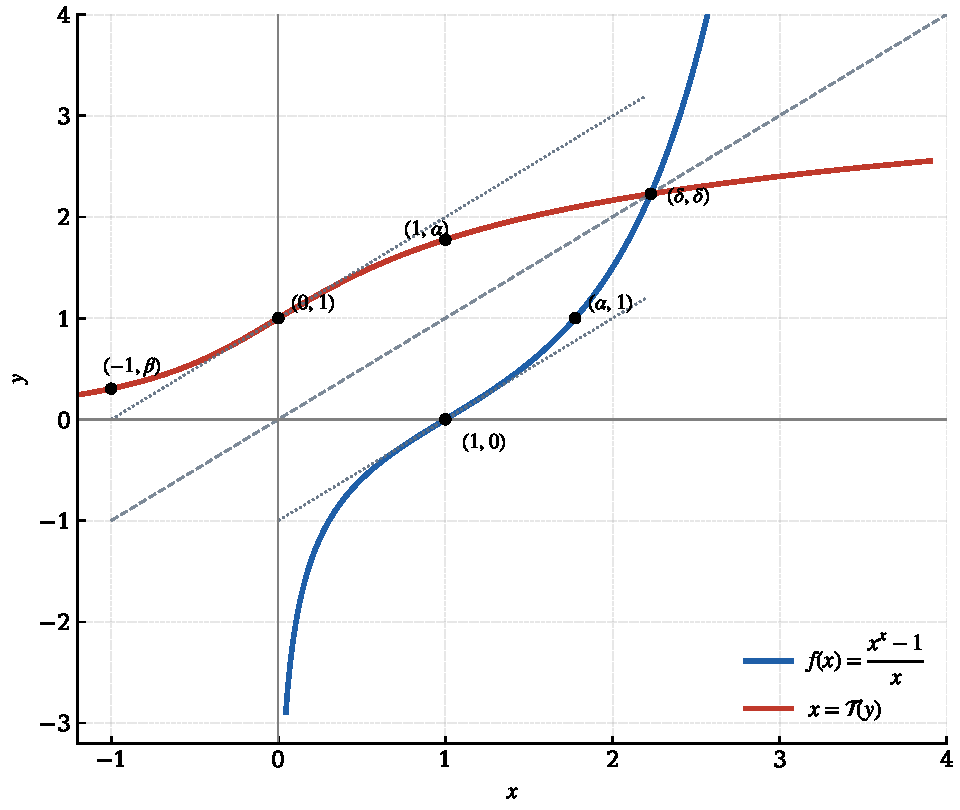
\includegraphics[width=0.78\textwidth]{figures/fig1_mirror.pdf}
    \caption{The forward map $f(x) = (x^{x}-1)/x$ (blue) and the Tahawus
    function $\Tah$ (red), mirror images across the diagonal (dashed).
    Dotted lines: the common tangent directions $y = x \mp 1$ at the
    reflected pair $(1,0)$--$(0,1)$. Marked points include
    $\alpha = \Tah(1)$, $\beta = \Tah(-1)$ and the fixed point
    $\delta$ of Section~\ref{sec:dynamics}.}
    \label{fig:mirror}
\end{figure}

\begin{proposition}[first derivatives and the reflected inflection]
\label{prop:derivatives}
Let $u := x - 1$. Then
\begin{equation}\label{eq:f-series}
    f(1+u) \;=\; u + \frac{u^{3}}{2} - \frac{u^{4}}{6} + \frac{u^{5}}{4} -
    \frac{7u^{6}}{40} + O(u^{7}) ,
\end{equation}
and consequently
\[
    f'(1) = 1,\qquad f''(1) = 0,\qquad f'''(1) = 3,\qquad f''''(1) = -4,
\]
while for the inverse function,
\[
    \Tah(0) = 1,\quad
    \Tah'(0) = 1,\quad
    \Tah''(0) = 0,\quad
    \Tah'''(0) = -3,\quad
    \Tah''''(0) = 4 .
\]
Both $f$ and $\Tah$ have an inflection at the reflected pair
$(1,0)$, $(0,1)$, with common tangent directions of slope exactly $1$.
\end{proposition}

\begin{proof}
Expanding $(1+u)\ln(1+u) = u + \tfrac{u^{2}}{2} - \tfrac{u^{3}}{6} +
\tfrac{u^{4}}{12} - \cdots$ and exponentiating,
\[
    (1+u)^{1+u} \;=\; 1 + u + u^{2} + \frac{u^{3}}{2} + \frac{u^{4}}{3} +
    O(u^{5}) ,
\]
whence, dividing by $1+u$,
\[
    \frac{(1+u)^{1+u} - 1}{1+u}
    \;=\; u + \frac{u^{3}}{2} - \frac{u^{4}}{6} + \frac{u^{5}}{4} -
    \frac{7u^{6}}{40} + O(u^{7}) ,
\]
(the quadratic term cancels). The derivative statements for $f$ follow
by comparing coefficients, since $f'(1+u) = 1 + \tfrac32 u^{2} -
\tfrac{2}{3}u^{3} + O(u^{4})$ shows $f''(1) = 0$ directly. For the
inverse, use $\Tah'(0) = 1/f'(1) = 1$,
$\Tah''(y) = -f''(x)/f'(x)^{3}$ and
$\Tah'''(y) = -f'''(x)/f'(x)^{3} + 3f''(x)^{2}/f'(x)^{5}$
(evaluated at $x = \Tah(y)$, all at $x = 1$), giving $\Tah'''(0) = -3$;
the value $\Tah''''(0) = 4$ is read off the reversion series of
Theorem~\ref{thm:maclaurin}. The inflection claim follows from
$f''(1) = 0 < f'''(1)$ and its mirrored statement, and the tangent
lines are $y = x - 1$ (for $f$ at $(1,0)$) and its reflection
$y = x + 1$ (for $\Tah$ at $(0,1)$).
\end{proof}

% =====================================================================
\section{The Tahawus constant: transcendence and arithmetic}
\label{sec:constant}
% =====================================================================

With the function firmly in place we turn to arithmetic. The key
observation is that the equation $x^{x} = bx+1$ is \emph{irrationality
rigid}: on rational inputs $x$, the power $x^{x}$ is rational only in
the trivial case.

\begin{lemma}\label{lem:irrational}
If $x = p/q \in \Q_{>0}$ in lowest terms with $q \ge 2$, then
$x^{x} \notin \Q$.
\end{lemma}

\begin{proof}
Suppose $(p/q)^{p/q} = m/n$ with $\gcd(m,n) = 1$. Raising to the
$q$-th power, $p^{p} n^{q} = m^{q} q^{p}$. Let $\ell$ be any prime
divisor of $q$ (one exists since $q \ge 2$). Since $\gcd(p,q) = 1$,
$\ell \nmid p$, and comparing $\ell$-adic valuations of both sides gives
\[
    q\, v_\ell(n) \;=\; q\, v_\ell(m) + p\, v_\ell(q),
\]
so $q$ divides $p\,v_\ell(q)$; as $\gcd(p,q)=1$, $q \mid
v_\ell(q)$. But $1 \le v_\ell(q) \le \log_{2} q < q$ for every $q \ge 2$,
a contradiction.
\end{proof}

\begin{theorem}[transcendence classification on rational arguments]
\label{thm:transcendence}
Let $b \in \Q$. Then $\Tah(b)$ is either a positive integer or a
transcendental number. The first alternative holds if and only if
\[
    b \;=\; \frac{n^{n} - 1}{n} \qquad\text{for some } n \in \N
    \qquad(\text{then } \Tah(b) = n),
\]
and the parameter value $b \mapsto \tfrac{n^{n}-1}{n}$ is strictly
increasing in $n$, so $n$ is unique.
\end{theorem}

\begin{proof}
Write $x = \Tah(b) > 0$, so that $x^{x} = bx + 1 \in \Q$.
If $x$ is rational, say $x = p/q$ in lowest terms, then $q = 1$ by
Lemma~\ref{lem:irrational} (otherwise $x^{x}$ would be irrational while
$bx+1$ is rational); thus $x = n \in \N$ and
$b = (n^{n} - 1)/n$. If instead $x$ is an algebraic irrational, then
$x \notin \{0,1\}$ (the case $x = 1$ forces $b = 0$, which returns
$x = \Tah(0) = 1$, rational, already covered), and the
Gelfond--Schneider theorem \cite{gelfond} applies: for algebraic
$\alpha_{0} \notin \{0,1\}$ and algebraic irrational $\beta_{0}$,
every value of $\alpha_{0}^{\beta_{0}}$ is transcendental. With
$\alpha_{0} = \beta_{0} = x$ we conclude that $x^{x}$ is transcendental,
contradicting $x^{x} = bx + 1 \in \Q$. Hence $x$ is transcendental.
Monotonicity of $n \mapsto n^{n-1} - \tfrac1n$ on $\N$ gives the
uniqueness of $n$.
\end{proof}

\begin{corollary}[Stanley's theorem, and more]\label{cor:stanley}
The Tahawus constant
\[
    \alpha \;=\; \Tah(1)
    \;=\; 1.7767750400970546974797307440387567486374110343292961390843740\ldots
\]
and the constant
\[
    \beta \;:=\; \Tah(-1)
    \;=\; 0.3036591270299660512450189512132226599911996187611727096441703\ldots
\]
(catalogued as \textrm{A226568} in the OEIS)
are transcendental. More generally $\Tah(b)$ is transcendental for every
rational $b \notin \bigl\{\tfrac{n^{n}-1}{n} : n \in \N\bigr\}$, while
$\Tah(0) = 1$, $\Tah\bigl(\tfrac32\bigr) = 2$,
$\Tah\bigl(\tfrac{26}{3}\bigr) = 3$, $\dots$ are integers.
\end{corollary}

\begin{proof}
The set $\bigl\{\tfrac{n^{n}-1}{n}\bigr\}$ equals
$\{0, \tfrac32, \tfrac{26}3, \tfrac{255}4, \ldots\}$; it is strictly
increasing starting at $0$, so it contains neither $1$ nor $-1$.
Apply Theorem~\ref{thm:transcendence}.
\end{proof}

\begin{remark}[history and credits]
\label{rem:stanley}
The transcendence of $\alpha$ was first proved by R.~P.~Stanley and
published as \emph{Quickie 88-10} in the Mathematical Entertainments
column of the \emph{Mathematical Intelligencer} \cite{stanley89}; the
proof is precisely the two-step exclusion above (Gelfond--Schneider plus
a rational-root argument), as recorded in the OEIS entry
\textrm{A124930} \cite{a124930}. The blog post \cite{blog} that
introduced the Tahawus function credits Stanley's result and adopts his
childhood town as the name. The transcendence of the companion constant
$\beta$'s affine image $v = 1/\beta - 1 = 2.2931662874\ldots$ was
independently obtained by Lord \cite{lord} in the \emph{Mathematical
Gazette}, under the equivalent equation $x = (1+1/x)^{x}$; it is
recovered by Corollary~\ref{cor:stanley} since $v$ is a rational
function of $\beta$ (see Theorem~\ref{thm:network} below). A pleasant
 curiosity recorded in \textrm{A124930} (G.~McGarvey, 2008): since
$\alpha^{\alpha - 1} = 1 + \tfrac1\alpha$, the constant $\alpha$ is a
fixed point of the nesting $x \mapsto \bigl(1 + 1/x\bigr)^{1/(\alpha-1)}$.
\end{remark}

\begin{remark}[complex roots are transcendental too]
\label{rem:complex-roots}
The Gelfond--Schneider step of Theorem~\ref{thm:transcendence} does not
use real-valuedness. If $z \in \C$ is an \emph{algebraic irrational}
solution of $z^{z} = z + 1$ (for any branch of the power), then
$z \notin \{0,1\}$ and $z^{z}$ is transcendental in every branch,
contradicting $z + 1$ algebraic. Rational solutions must be real (a
branch value $z^{z}$ equal to the real number $z+1>0$ forces the real
branch), and these are excluded by Lemma~\ref{lem:irrational} for
non-integers and by direct inspection for integers. Hence \emph{every}
complex solution of $z^{z} = z+1$ is transcendental. We do not know how
many complex solutions there are (see
Open Problem~\ref{op:complex-roots}).
\end{remark}

% =====================================================================
\section{The sandwich theorem}\label{sec:sandwich}
% =====================================================================

The exponential $\ee^{y}$ and the line $1+y$ share the value $1$ and the
slope $1$ at $y = 0$, and $\ee^{y} \ge 1 + y$ everywhere. The Tahawus
function shares both normalization properties---$\Tah(0) = 1$,
$\Tah'(0) = 1$---and the next theorem shows that it \emph{threads
between} the two classical curves. Each of the three inequalities has a
one-line proof, which is part of the charm.

\begin{theorem}[sandwich theorem]\label{thm:sandwich}
\begin{enumerate}[label=\textup{(\roman*)}, leftmargin=2.4em]
    \item For all $y \ne 0$: $\Tah(y) < \ee^{y}$.
    \item For all $y > 0$: $\Tah(y) < 1 + y$.
    \item For all $-1 < y < 0$: $1 + y < \Tah(y)$
    (and, trivially, $\Tah(y) < \ee^{y}$ by (i)).
\end{enumerate}
In particular, on $(-1, 0)$ the Tahawus function squeezes between the
line and the exponential, $1 + y < \Tah(y) < \ee^{y}$, while on
$(0, \infty)$ it lies below both. Moreover
\[
    \frac{\Tah(y)}{\ee^{y}} \;\longrightarrow\; 1
    \quad (y \to -\infty),
\]
with the refinement
$\ln \Tah(y) = y - \tfrac{y^{2}}{2}\ee^{y}\bigl(1 + o(1)\bigr)$
(Theorem~\ref{thm:asymptotics}).
\end{theorem}

\begin{proof}
Since $f$ is strictly increasing (Theorem~\ref{thm:bijection}),
inequalities between $\Tah$ and a candidate value $g(y)$ can be tested
by applying $f$ to both sides whenever $g(y) > 0$.

(i) $\Tah(y) < \ee^{y} \iff y < f(\ee^{y})$. Now
$f(\ee^{y}) = \bigl(\ee^{y\ee^{y}} - 1\bigr)\ee^{-y}$, so
$y < f(\ee^{y}) \iff y\ee^{y} < \ee^{y\ee^{y}} - 1 \iff
1 + y\ee^{y} < \ee^{y\ee^{y}}$, which is the strict convexity inequality
$1 + w < \ee^{w}$ at $w = y\ee^{y} \ne 0$ (note $w = 0$ only at
$y = 0$).

(ii) For $y > 0$: $\Tah(y) < 1 + y \iff y < f(1+y) \iff
(1+y)^{1+y} > 1 + y + y^{2}$. If $0 < y < 1$, then
\[
    (1+y)^{y} \;=\; \ee^{y \ln(1+y)}
    \;\ge\; \ee^{y(y - y^{2}/2)}
    \;\ge\; 1 + y^{2} - \tfrac{y^{3}}{2}
    \;>\; 1 + \frac{y^{2}}{1+y} ,
\]
where we used $\ln(1+y) \ge y - \tfrac{y^{2}}{2}$, then
$\ee^{u} \ge 1+u$, and finally $\bigl(1 - \tfrac{y}{2}\bigr)(1+y) > 1
\iff y(1-y) > 0$. Multiplying by $1+y$ gives
$(1+y)^{1+y} > 1 + y + y^{2}$. If $y \ge 1$, then
$(1+y)^{1+y} \ge (1+y)^{2} = 1 + 2y + y^{2} > 1 + y + y^{2}$.

(iii) Let $x := 1 + y \in (0, 1)$. Then
$\Tah(y) > 1 + y \iff f(x) < x - 1 \iff x^{x} < x^{2} - x + 1$. By the
weighted arithmetic--geometric mean inequality with weights
$x$ and $1-x$ applied to the two numbers $x$ and $1$,
\[
    x^{x}\cdot 1^{\,1-x} \;\le\; x\cdot x + (1-x)\cdot 1
    \;=\; x^{2} + 1 - x ,
\]
with equality only when the two weighted numbers coincide, i.e.\ at
$x = 1$; the inequality is strict on $(0,1)$.

Finally, for the limit as $y \to -\infty$, write $x = \Tah(y) \to 0^{+}$
and expand
\[
    y \;=\; \frac{x^{x} - 1}{x} \;=\; \ln x + \frac{x \ln^{2} x}{2} +
    O\bigl(x^{2}\ln^{3} x\bigr) ,
\]
so $y - \ln x = \tfrac{x}{2}\ln^{2}x\,(1 + o(1))$ with
$\ln x = y(1 + o(1))$, giving $\ln x - y = -\tfrac{y^{2}}{2}\ee^{y}
(1+o(1))$ since $x \sim \ee^{y}$. (A complete statement with proof is
Theorem~\ref{thm:asymptotics}.)
\end{proof}

Figure~\ref{fig:sandwich} displays the two sides of the sandwich: on the
left panel, $\Tah$ threads between $1+y$ and $\ee^{y}$ across
$(-1,0)$ and dips below $1+y$ afterwards; on the right panel, the ratio
$\Tah(y)/\ee^{y}$ is shown to climb to $1$ from below as
$y \to -\infty$, already indistinguishable from $1$ at $y = -20$ (at
$y = -40$ the relative deficit is $3.4 \times 10^{-15}$).

\begin{figure}[t]
    \centering
    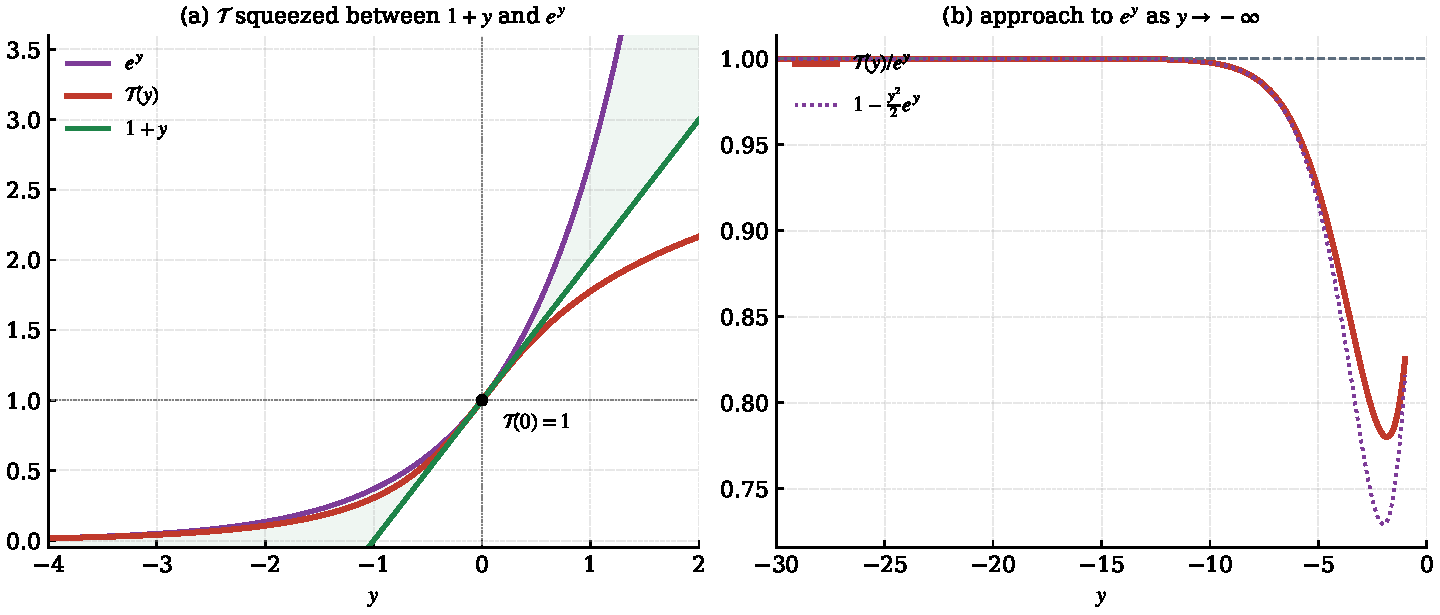
\includegraphics[width=0.98\textwidth]{figures/fig2_sandwich.pdf}
    \caption{(a) The sandwich of Theorem~\ref{thm:sandwich}: on
    $(-1,0)$, $1+y < \Tah(y) < \ee^{y}$ (shaded strip); for $y > 0$,
    $\Tah(y) < 1 + y < \ee^{y}$. (b) The ratio $\Tah(y)/\ee^{y}$
    (solid) against the asymptotic prediction
    $1 - \tfrac{y^{2}}{2}\ee^{y}$ of Theorem~\ref{thm:asymptotics}
    (dotted): the Tahawus function is an asymptotic copy of $\exp$
    on the far left.}
    \label{fig:sandwich}
\end{figure}

The exponential comparison can be sharpened to a Lipschitz statement:
the slope of $\Tah$ never exceeds $1$.

\begin{proposition}[$1$-Lipschitz property]\label{prop:lipschitz}
For all $y \in \R$,
\[
    0 \;<\; \Tah'(y) \;\le\; 1 ,
    \qquad\text{with equality iff } y = 0 .
\]
Equivalently, $f'(x) \ge 1$ for all $x > 0$ with equality only at
$x = 1$; hence $|\Tah(y_{1}) - \Tah(y_{2})| \le |y_{1} - y_{2}|$ for all
real $y_{1}, y_{2}$.
\end{proposition}

\begin{proof}
By \eqref{eq:x2fprime},
$x^{2}(f'(x) - 1) = h(x) := x^{x}(x\ln x + x - 1) + 1 - x^{2}$, so we
must show $h \ge 0$ on $(0,\infty)$ with equality only at $x = 1$. Put
$a := x \ln x$ and $m := x\ln x + x - 1 = a + x - 1$.

\emph{Case $x \ge 1$.} Then $a \ge 0$ and $m \ge 0$ (as $m(1) = 0$ and
$m' = \ln x + 2 > 0$ on $[1,\infty)$). Since $\ee^{a} \ge 1 + a$,
\[
    h \;\ge\; (1 + a)(a + x - 1) + 1 - x^{2}
    \;=\; x^{2}\ln x\,(\ln x + 1) + x - x^{2}
    \;=\; x\,p(x),
\]
where $p(x) := x\ln x\,(\ln x + 1) - x + 1$. Now
$p(1) = 0$ and $p'(x) = \ln x\,(\ln x + 3) \ge 0$ for $x \ge 1$, so
$p \ge 0$ on $[1,\infty)$, hence $h \ge 0$; equality forces $a = 0$
(i.e.\ $x = 1$) and $p(x) = 0$.

\emph{Case $0 < x < 1$.} Then $m < 0$ (as $m$ decreases from
$-1$ at $0^{+}$, has its minimum $-\ee^{-2} - 1 < 0$ at $x = \ee^{-2}$,
and returns to $m(1) = 0$ only at the endpoint). Since
$u := a = x\ln x \in (-\tfrac1\ee, 0)$ and $\ee^{u} \le \tfrac{1}{1-u}$
(the inequality $\ee^{-u} \ge 1 - u$ for $u < 1$), and since $m < 0$,
\[
    x^{x} m \;=\; \ee^{u}\,m \;\ge\; \frac{m}{1 - u} .
\]
Therefore
\[
    h \;\ge\; \frac{m}{1 - x\ln x} + 1 - x^{2}
    \;=\; \frac{x - x^{2} + x^{3}\ln x}{1 - x\ln x}
    \;=\; \frac{x\,r(x)}{1 - x\ln x},
\]
where $r(x) := 1 - x + x^{2}\ln x$. The denominator exceeds $1$, and
$r > 0$ on $(0,1)$: indeed $r(1) = 0$, $r(0^{+}) = 1$, and
$r'(x) = x(1 + 2\ln x) - 1 < 0$ on $(0,1)$ because the auxiliary
function $u_{1}(x) := x(1 + 2\ln x)$ satisfies $u_{1} \le 1$ on
$(0,1]$, with equality only at $x = 1$ (Lemma~\ref{lem:u1} in the
Appendix). Hence $r$ decreases strictly from $1$
to $0$ and is positive. This gives $h > 0$ on $(0,1)$, completing the
proof.
\end{proof}

\begin{remark}
Proposition~\ref{prop:lipschitz} says that $\Tah$ is a (weak)
contraction of the whole real line into the positive half-line. In
particular the graph of $\Tah$ is flatter than the diagonal everywhere
except at the origin, where it is tangent to it; this is visible in
Figure~\ref{fig:mirror} and is the mechanism behind the global dynamics
of Section~\ref{sec:dynamics}. Note the pleasing division of labour in
the proof: the elementary inequalities $\ee^{u} \ge 1 + u$ (for $u \ge
0$) and $\ee^{u} \le 1/(1-u)$ (for $u < 1$) each take care of one side
of $x = 1$.
\end{remark}

% =====================================================================
\section{Local theory: the Maclaurin expansion and the radius of
convergence}\label{sec:maclaurin}
% =====================================================================

The sandwich theorem controls the global position of $\Tah$; we now zoom
in on the origin, where the three normalizations
$\Tah(0) = \Tah'(0) = 1$, $\Tah''(0) = 0$ of
Proposition~\ref{prop:derivatives} suggest a degenerate local structure.
The degeneracy is real, and it is the entrance to a chain of
consequences: an inflection with third-order contact, a clean
convexity dichotomy, and a Maclaurin series whose radius of convergence
is set by a pair of complex critical values of $f$, reached through a
picture (Figure~\ref{fig:slit}) that we find to be one of the prettiest
by-products of the theory.

\subsection{The series}

\begin{theorem}[Maclaurin expansion; the quadratic term vanishes]
\label{thm:maclaurin}
The Tahawus function is real-analytic at the origin, and
\begin{equation}\label{eq:maclaurin}
\begin{split}
    \Tah(y) \;=\; 1 + y - \frac{y^{3}}{2} + \frac{y^{4}}{6} +
    \frac{y^{5}}{2} - \frac{49\,y^{6}}{120} - \frac{5\,y^{7}}{9} \\[2mm]
    \qquad + \frac{4313\,y^{8}}{5040} + \frac{49\,y^{9}}{90} -
    \frac{6341\,y^{10}}{3780} - \frac{11549\,y^{11}}{50400} +
    \frac{62041117\,y^{12}}{19958400} + O(y^{13}) .
\end{split}
\end{equation}
In particular the coefficient of $y^{2}$ vanishes identically: $\Tah$
has third-order contact with its tangent line $1+y$ at the origin.
All coefficients are rational numbers.
\end{theorem}

\begin{proof}
Write $u := x - 1$ and recall from \eqref{eq:f-series} that
\begin{equation}\label{eq:phi-def}
    y \;=\; f(1+u) \;=\; u\,\varphi(u),
    \qquad
    \varphi(u) \;:=\; \frac{f(1+u)}{u}
    \;=\; 1 + \frac{u^{2}}{2} - \frac{u^{3}}{6} + \frac{u^{4}}{4} -
    \frac{7u^{5}}{40} + \cdots,
\end{equation}
a power series with $\varphi(0) = f'(1) = 1 \ne 0$. The
Lagrange--B\"urmann inversion formula applied to $y = u\,\varphi(u)$
gives
\begin{equation}\label{eq:lagrange}
    u(y) \;=\; \sum_{n \ge 1} \frac{y^{n}}{n}\,
    [u^{\,n-1}]\,\varphi(u)^{-n},
    \qquad\text{so that}\qquad
    \Tah(y) \;=\; 1 + \sum_{n \ge 1} d_{n} y^{n},
    \quad d_{n} := \frac{1}{n}[u^{\,n-1}]\,\varphi(u)^{-n},
\end{equation}
with positive radius of convergence, since $\varphi(0) \ne 0$. Each
$d_n$ is a rational number, because the coefficients of $\varphi$ are
rational: they are obtained from the exact expansion
$E(u) := (1+u)\ln(1+u) = \sum_{k\ge1} (-1)^{k+1}u^{k}/(k(k-1))$ by
exponentiating ($x^{x} = \exp E$), dividing by $1+u$, and reverting;
all steps are rational recurrences, reproduced in
Appendix~\ref{sec:computational}, which is how the twelve coefficients
displayed in \eqref{eq:maclaurin} were computed exactly. The vanishing
of $d_2$ was already proved in Proposition~\ref{prop:derivatives} via
$\Tah''(0) = -f''(1)/f'(1)^{3} = 0$; it can also be read off directly
from \eqref{eq:phi-def}, since $\varphi$ itself has no linear term, so
$\varphi^{-2}$ has no $u^{1}$-term. As a numerical check, the partial
sum of \eqref{eq:maclaurin} through $y^{12}$ was evaluated against the
directly computed value of $\Tah$: the differences are
$3.2 \times 10^{-11}$ at $y = 0.15$, $3.3 \times 10^{-7}$ at
$y = 0.3$ and $7.0 \times 10^{-5}$ at $y = 0.45$, consistent with a
twelve-term truncation of a series of radius $R \approx 0.65$
(Subsection~\ref{subsec:radius} below).
\end{proof}

\begin{remark}[why the quadratic term vanishes]\label{rem:why-vanishing}
The cancellation has a transparent cause in the two-term decomposition
\eqref{eq:f-two-terms}, $f(x) = x^{x-1} - 1/x$. At $x = 1+u$,
\[
    x^{x-1} \;=\; (1+u)^{u} \;=\; \exp\!\bigl(u\ln(1+u)\bigr)
    \;=\; 1 + 0\cdot u + u^{2} - \frac{u^{3}}{2} + \cdots,
    \qquad
    \frac{1}{x} \;=\; 1 - u + u^{2} - \cdots,
\]
and the two terms have \emph{identical quadratic parts} $+u^{2}$, which
cancel in the difference, while their linear parts differ by exactly
$u$. So $f$ is ``linear plus cubic'' at $x=1$, and reversion preserves
the pattern: $\Tah$ is ``linear plus cubic'' at $y = 0$. Neither
$\ee^{y}$ nor $1 + y + cy^{2}$ with $c \ne 0$ shares this property; in
the two-parameter family of functions with $\Tah(0)=\Tah'(0)=1$ the
Tahawus function sits on the measure-zero slice $c = 0$.
\end{remark}

\subsection{Convexity dichotomy}

The sign of $\Tah''$ is the mirror of the sign of $f''$, and $f''$ has
an entirely explicit form which behaves differently on the two sides of
$x = 1$.

\begin{theorem}[convexity dichotomy]\label{thm:convexity}
The Tahawus function is strictly convex on $(-\infty, 0)$ and strictly
concave on $(0, \infty)$; equivalently, $f$ is strictly concave on
$(0,1)$ and strictly convex on $(1,\infty)$. The point $(0,1)$ is the
unique inflection point of $\Tah$, and there the tangent line $1 + y$
has contact of order three.
\end{theorem}

\begin{proof}
Differentiating \eqref{eq:fprime},
\begin{equation}\label{eq:fprimeprime}
    f''(x) \;=\; x^{x-1}\Bigl(\ln x + 1 - \frac{1}{x}\Bigr)^{2}
    \;+\; \frac{x^{x}(x+1) - 2}{x^{3}} .
\end{equation}
For $x > 1$ we have $x^{x} > 1$ and $x + 1 > 2$, so the second term is
positive and the first is nonnegative: $f'' > 0$.

For $0 < x < 1$, substitute $x = \ee^{-s}$, $s > 0$, and write
$E := \ee^{-s} = x$ and $t := (s-1)E$. Using
$\ln x + 1 - \tfrac1x = -(1+t)/E$ and $x^{x+2} = \ee^{-sE}E^{2}$, a
direct substitution into \eqref{eq:fprimeprime} gives the identity
\begin{equation}\label{eq:psi-identity}
    f''(x)\,x^{3} \;=\; \Psi(s) - 2,
    \qquad
    \Psi(s) \;:=\; \ee^{-sE}\Bigl[\bigl(1 + t\bigr)^{2} + 1 + E\Bigr],
    \qquad t = (s-1)\ee^{-s},
\end{equation}
which we verified numerically to fifty digits at several points. Now
$(1+t)^{2} + 1 + E = 2 + w$ with $w := 2t + t^{2} + E$. Since
$h(s) := (s-1)\ee^{-s} > -1$ for $s > 0$ (Lemma~\ref{lem:q}(i) in the
appendix), we have $w \ge (1+t)^{2} - 1 + E > -1$, so $2 + w > 1 > 0$
and $v := w/2 > -\tfrac12$; the elementary bound
$\ln(2+w) = \ln 2 + \ln(1+v) \le \ln 2 + v$ therefore applies, and
\[
    \ln \Psi
    \;=\; -sE + \ln(2 + w)
    \;\le\; \ln 2 - sE + t + \frac{t^{2}}{2} + \frac{E}{2}
    \;=\; \ln 2 + \frac{E}{2}\Bigl((s-1)^{2}E - 1\Bigr)
    \;<\; \ln 2 ,
\]
the last inequality being Lemma~\ref{lem:q}(ii):
$(s-1)^{2}\ee^{-s} < 1$ for all $s > 0$. Hence $\Psi < 2$ and
$f''(x) < 0$ on $(0,1)$. Since
$\Tah''(y) = -f''\bigl(\Tah(y)\bigr)/f'\bigl(\Tah(y)\bigr)^{3}$ and
$\Tah(y) < 1 \iff y < 0$, the claims follow; the inflection statement
is Proposition~\ref{prop:derivatives} plus the sign change just
established.
\end{proof}

\subsection{The radius of convergence and the slit}\label{subsec:radius}

The series \eqref{eq:maclaurin} cannot converge everywhere: $\Tah$ has
finite limits of slope, but the complex continuation of $f$ has
critical points, and critical values of $f$ are branch points of
$\Tah$. By \eqref{eq:x2fprime}, the critical points of $f$ are the
zeros of
\begin{equation}\label{eq:G-def}
    G(x) \;:=\; x^{x+1}\Bigl(\ln x + 1 - \frac{1}{x}\Bigr) + 1
    \qquad\bigl(= x^{2} f'(x)\bigr),
\end{equation}
and $G$ has none on the positive real axis (Theorem~\ref{thm:bijection}).
Solving $G = 0$ in the complex plane (principal branch of the power) by
path continuation combined with Newton iteration, starting from the
direction suggested by the coefficients themselves, locates a conjugate
pair of critical points
\begin{align*}
    x_{c} \;&=\; 0.72822912959789 \;\pm\; 1.1414509801214\,i, \\
    y_{c} \;&=\; f(x_{c}) \;=\; -0.10489522487779 \;\pm\; 0.64412488108293\,i,
\end{align*}
(the signs being paired), at distance
\begin{equation}\label{eq:R-value}
    R \;:=\; |y_{c}| \;=\; 0.6526100448\ldots
\end{equation}
from the origin. A broad sweep of initial conditions for the Newton
iteration found no closer critical values; the next nearest lies near
the logarithmic singularity of $f$ at $x = 0$, at modulus $\approx
104.9$, and plays no role. Two independent cross-checks corroborate
\eqref{eq:R-value}. First, fitting the dominant conjugate-pair pattern
$d_{n} \sim A\lambda^{n} + \overline{A}\,\overline{\lambda}^{n}$ (that
is, $d_{n+2} = S d_{n+1} - P d_{n}$) to the sixty exact rational
coefficients by least squares yields a singularity estimate of modulus
$0.6698$, within three percent of \eqref{eq:R-value}; naive ratio
estimates $|d_{n}/d_{n+1}|$ are useless here because the dominant
singularity is complex, so the ratios oscillate between $0.07$ and $7$
instead of converging. Second, the partial sums of \eqref{eq:maclaurin}
behave differently on the two sides of $R$ (Table~\ref{tab:partials}):
at $0.9R$ the truncation error decreases steadily with the number of
terms, while at $1.06R$ it stagnates and oscillates, never falling
below forty-five times the best inside value.

\begin{table}[t]
\centering
\caption{Partial sums $S_{n}(y)$ of \eqref{eq:maclaurin} inside and
outside the radius: $|S_{n}(y) - \Tah(y)|$. Inside $R$ the error decays
geometrically; outside it does not decay at all.}
\label{tab:partials}
\begin{tabular}{rcc}
\toprule
$n$ & $\quad |S_{n}(0.9R) - \Tah(0.9R)|\quad$ & $\quad |S_{n}(1.06R) - \Tah(1.06R)|\quad$ \\
\midrule
$8$  & $1.3 \times 10^{-3}$ & $7.6 \times 10^{-3}$ \\
$12$ & $2.3 \times 10^{-3}$ & $1.9 \times 10^{-2}$ \\
$16$ & $1.3 \times 10^{-3}$ & $2.0 \times 10^{-2}$ \\
$20$ & $5.3 \times 10^{-4}$ & $1.5 \times 10^{-2}$ \\
$24$ & $1.1 \times 10^{-4}$ & $4.7 \times 10^{-3}$ \\
\bottomrule
\end{tabular}
\end{table}

We summarize the state of knowledge as follows: the Maclaurin series of
$\Tah$ has radius of convergence $R = 0.6526100\ldots$, the nearest
singularities being the conjugate critical values of $f$ above, at
which the inverse function develops square-root branch points. The
determination of $R$ is numerical (two independent methods agree), and
promoting it to a proof is Open Problem~\ref{op:radius}.

Figure~\ref{fig:slit} explains, at the same time, what the complex
branch cut of $\Tah$ looks like. Let $\gamma^{+}$ be the image of the
negative real axis under the principal-branch continuation of $f$,
\[
    \gamma^{+} \;:=\; \bigl\{\, f(-r) \;:\; r > 0 \,\bigr\},
    \qquad
    f(-r) \;=\; \frac{(-r)^{-r} - 1}{-r}
    \;=\; \frac{1 - r^{-r}\ee^{-i\pi r}}{r} ,
\]
together with its conjugate $\overline{\gamma^{+}}$. As
$r \to 0^{+}$ the curve escapes to $-\infty$ at height $\pi$, and as
$r \to \infty$ it spirals into the origin: the phase $-i\pi r$ rotates
faster and faster while the amplitude $r^{-r}$ collapses, so the curve
winds through decreasing circles, crossing the real axis exactly at
the integer parameters $r = n$, where
\begin{equation}\label{eq:bn-on-slit}
    f(-n) \;=\; \frac{1 - (-1)^{n} n^{-n}}{n} \;=\; b_{n},
\end{equation}
a \emph{rational} number (Theorem~\ref{thm:negroots} below proves these
are the only rational points of the slit). The points $b_n$ alternate
around $1/n$: $b_n > 1/n$ for $n$ odd, $b_n < 1/n$ for $n$ even, and
$b_{n} \to 0$. The critical values $y_{c}, \overline{y_{c}}$ responsible
for the radius \eqref{eq:R-value} sit just inside the first turn of the
spiral, on either side of the real axis, at the squares marked in the
figure; the dotted circle is $|y| = R$.

\begin{figure}[t]
    \centering
    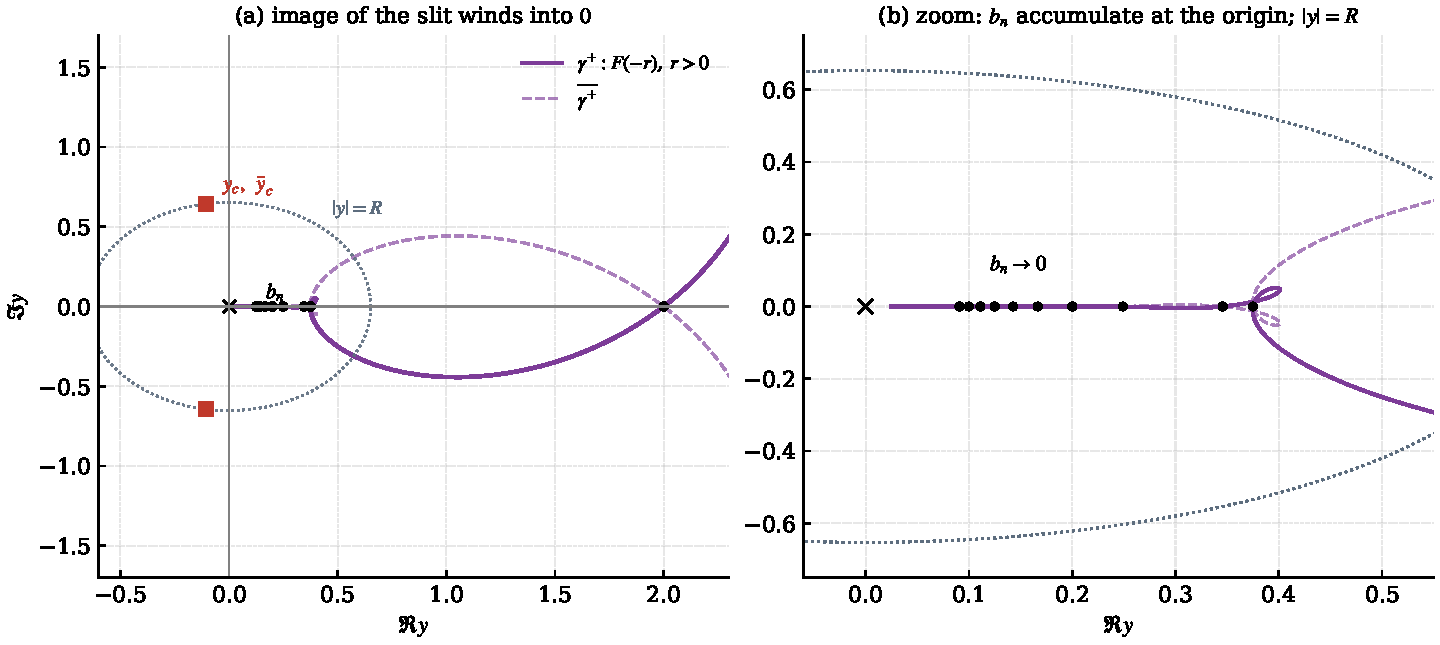
\includegraphics[width=0.98\textwidth]{figures/fig4_slit.pdf}
    \caption{(a) The slit $\gamma^{+} = f((-\infty,0))$ (solid) and its
    conjugate (dashed): the image of the negative real axis under $f$
    spirals from $-\infty + i\pi$ into the origin, crossing the real
    axis exactly at the rational points $b_{n} = (1-(-1)^{n}n^{-n})/n$
    (dots). The critical values $y_{c}$, $\overline{y_{c}}$ (squares)
    lie at distance $R = 0.6526\ldots$ from the origin (dotted circle)
    and bound the disk of convergence of the Maclaurin series
    \eqref{eq:maclaurin}. (b) Zoom near the origin: the crossings
    $b_{n}$ accumulate at $0$ alternately from both sides of $1/n$.}
    \label{fig:slit}
\end{figure}

% =====================================================================
\section{Special values, the golden comparison, and the OEIS
constellation}\label{sec:values}
% =====================================================================

Theorem~\ref{thm:transcendence} described the arithmetic of $\Tah(b)$
for rational $b$ in bulk; this section exhibits the concrete specimens.
Three families of exact values exist---integers, unit fractions, and
negative integers---and around them a constellation of five constants
has accumulated in the On-Line Encyclopedia of Integer Sequences, tied
together by elementary but pleasing identities.

\subsection{Exact values}

\begin{proposition}[exact values]\label{prop:exactvalues}
For every $n \in \N$,
\begin{equation}\label{eq:exact-families}
    \Tah\Bigl(\frac{n^{n}-1}{n}\Bigr) = n,
    \qquad
    \Tah\Bigl(n^{\,1-\frac{1}{n}} - n\Bigr) = \frac{1}{n} .
\end{equation}
The first family starts $0, \tfrac32, \tfrac{26}{3}, \tfrac{255}{4},
\tfrac{3124}{5},\ldots$ (at $x = 1,2,3,4,5,\ldots$); the second starts
$\sqrt2 - 2,\; 3^{2/3} - 3,\; 4^{3/4} - 4 = 2\sqrt2 - 4,\ldots$ (at
$x = \tfrac12, \tfrac13, \tfrac14, \ldots$). Together with
interpolation, these are the only rational arguments $b$ for which
$\Tah(b)$ is rational or algebraic (Theorem~\ref{thm:transcendence}).
\end{proposition}

\begin{proof}
Both identities are the statement $f(x) = b$ at $x = n$ and
$x = 1/n$: indeed $f(n) = (n^{n}-1)/n$, and
\[
    f\Bigl(\frac1n\Bigr) \;=\; \frac{(1/n)^{1/n} - 1}{1/n}
    \;=\; n \cdot \bigl(n^{-1/n} - 1\bigr)
    \;=\; n^{\,1-1/n} - n ,
\]
where $n^{\,1-1/n} = (n^{n-1})^{1/n}$ is the surd displayed. The
exactness was verified symbolically for $n \le 7$ and numerically to
eighty digits.
\end{proof}

The surd family gives $\Tah$ a supply of algebraic \emph{inputs} with
algebraic \emph{outputs}---$\Tah$ is not a transcendence machine
everywhere, only on the rational arguments off the two lattices
\eqref{eq:exact-families}. For instance
$\Tah(\sqrt2 - 2) = \tfrac12$ exactly, while $\Tah(-0.6)$, a
millimeter to the left on the $b$-axis, is transcendental.

\subsection{The golden comparison}

The quadratic pencil $x^{2} = bx + 1$ has positive root
$\varphi_b = (b + \sqrt{b^{2}+4})/2$, the family of metallic means
containing the golden ratio $\varphi = \varphi_1$. The super-quadratic
pencil has positive root $\Tah(b)$. The comparison between the two
turns out to be a \emph{single sign computation}.

\begin{theorem}[golden comparison]\label{thm:golden}
For all real $b$,
\[
\begin{aligned}
    \Tah(b) > \varphi_b \;&\iff\; 0 < b < \frac32,
    \qquad
    \Tah(b) = \varphi_b \iff b \in \Bigl\{0, \frac32\Bigr\},\\[1mm]
    \Tah(b) < \varphi_b \;&\iff\; b < 0 \text{ or } b > \frac32 .
\end{aligned}
\]
The two exact coincidences are $\Tah(0) = \varphi_{0} = 1$ and
$\Tah(\tfrac32) = \varphi_{3/2} = 2$.
\end{theorem}

\begin{proof}
Since $f$ is strictly increasing, $\Tah(b) > \varphi_b$ is equivalent
to $f(\varphi_b) < b$. But $\varphi_b$ solves $x^{2} = bx+1$, i.e.\
$b = \varphi_b - 1/\varphi_b$; therefore
\[
    f(\varphi_b) - b
    \;=\; \Bigl(\varphi_b^{\,\varphi_b - 1} - \frac{1}{\varphi_b}\Bigr)
    - \Bigl(\varphi_b - \frac{1}{\varphi_b}\Bigr)
    \;=\; \varphi_b^{\,\varphi_b - 1} - \varphi_b
    \;=\; \varphi_b \bigl(\varphi_b^{\,\varphi_b - 2} - 1\bigr),
\]
whose sign is the sign of $(\varphi_b - 2)\ln\varphi_b$. As
$b \mapsto \varphi_b$ is an increasing bijection $\R \to (0,\infty)$
with $\varphi_0 = 1$ and $\varphi_{3/2} = 2$, the sign is positive
exactly for $1 < \varphi_b < 2$, i.e.\ $0 < b < \tfrac32$, zero exactly
at $\varphi_b \in \{1,2\}$, and negative on the two outside intervals.
\end{proof}

\begin{remark}
The coincidence set $\{0, \tfrac32\}$ reflects the accident
$n^{n} = n^{2}$, which holds \emph{only} for $n \in \{1,2\}$: the
super-square and the square agree at $1$ and $2$ and nowhere else. It
is pleasant that the two most famous members of the two pencils---the
golden ratio and the Tahawus constant---obey
$\varphi < \alpha = \Tah(1) = 1.7767\ldots$, and that the ``excess''
$\Tah(b) - \varphi_b$, which vanishes at both ends of
$(0,\tfrac32)$, peaks at about $0.19000\ldots$ near $b \approx 0.7$
(between the rows $0.5$ and $1$ of Table~\ref{tab:golden}).
\end{remark}

\begin{table}[t]
\centering
\small
\caption{The Tahawus root versus the metallic root of the same
super-quadratic/quadratic $b$. The difference vanishes exactly at
$b = 0$ and $b = 3/2$ and changes sign there.}
\label{tab:golden}
\begin{tabular}{rrrr}
\toprule
$b$ & $\Tah(b)$ & $\varphi_b$ & $\Tah(b) - \varphi_b$ \\
\midrule
$-1$    & $0.3036591$  & $0.6180340$  & $-0.3143749$ \\
$-0.5$  & $0.5565737$  & $0.7807764$  & $-0.2242027$ \\
$0.5$   & $1.4559593$  & $1.2807764$  & $+0.1751828$ \\
$1$     & $1.7767750$  & $1.6180340$  & $+0.1587411$ \\
$1.4$   & $1.9609108$  & $1.9206556$  & $+0.0402552$ \\
$1.49$  & $1.9961956$  & $1.9920064$  & $+0.0041892$ \\
$1.5$   & $2.0000000$  & $2.0000000$  & $0$ \\
$1.51$  & $2.0037821$  & $2.0080064$  & $-0.0042243$ \\
$2$     & $2.1657594$  & $2.4142136$  & $-0.2484542$ \\
$3$     & $2.4019926$  & $3.3027756$  & $-0.9007830$ \\
$10$    & $3.0770622$  & $10.0990195$ & $-7.0219573$ \\
\bottomrule
\end{tabular}
\end{table}

\subsection{Negative integer roots, and the census of real roots}
\label{subsec:negative}

For negative $x$ the power $x^{x}$ is multivalued; we use the
principal branch $x^{x} = \exp(x \Log x)$, under which $x^{x}$ is real
precisely for negative integers (this is the branch plotted in
Figure~\ref{fig:slit}). The defining equation of the super-quadratic
then admits a second, exactly solvable family.

\begin{theorem}[negative integer roots]\label{thm:negroots}
\begin{enumerate}[label=\textup{(\roman*)}, leftmargin=2.4em]
\item For every $n \in \N$, the negative integer $x = -n$ solves
\[
    x^{x} \;=\; b_{n}\,x + 1
    \qquad\text{with}\qquad
    b_{n} \;:=\; \frac{1 - (-1)^{n}\, n^{-n}}{n} \;\in\; \Q ,
\]
e.g.\ $(-1)^{-1} = -1 = 2\cdot(-1) + 1$ (so $b_1 = 2$),
$(-2)^{-2} = \tfrac14 = \tfrac38 \cdot (-2) + 1$, and the sequence
$b_{n} = 2, \tfrac38, \tfrac{28}{81}, \tfrac{255}{1024}, \ldots$
alternates around $1/n$ and tends to $0$.
\item On the principal branch, $f(-r)$ is real \emph{if and only if}
$r \in \N$; hence the points \eqref{eq:bn-on-slit} are exactly the real
points of the slit $\gamma^{+} \cup \overline{\gamma^{+}}$ of
Figure~\ref{fig:slit}.
\item $\alpha$ is the unique \emph{real} root of $x^{x} = x + 1$ in
either convention for negative powers (principal branch, or the
real-branch convention $(-p/q)^{-p/q} := \bigl((-p/q)^{-p}\bigr)^{1/q}$
with $q$ odd).
\end{enumerate}
\end{theorem}

\begin{proof}
(i) $(-n)^{-n} = (-1)^{n} n^{-n}$, and
$(-1)^{n}n^{-n} = b_{n} \cdot (-n) + 1$ rearranges to
$b_{n} = (1 - (-1)^{n}n^{-n})/n$; these are rational, and the
identities were verified symbolically for $n \le 7$.

(ii) On the principal branch $(-r)^{-r} =
\exp\bigl(-r\ln r - i\pi r\bigr) = r^{-r}\ee^{-i\pi r}$, so
\[
    f(-r) \;=\; \frac{(-r)^{-r} - 1}{-r}
    \;=\; \frac{1 - r^{-r}\ee^{-i\pi r}}{r} ,
\]
which is real iff $\ee^{-i\pi r}$ is real, i.e.\ iff $\sin(\pi r) =
0$, i.e.\ iff $r \in \Z$; positivity of $r$ gives $r \in \N$. Then
\eqref{eq:bn-on-slit} applies.

(iii) On the principal branch, $x^{x} \in \R$ for $x < 0$ only at the
integers (part (ii)), and $x = -n$ solves $x^{x} = x + 1$ only if
$b_{n} = 1$, which never happens: $b_{1} = 2$, and for $n \ge 2$,
$b_{n} \le (1 + 2^{-2})/n \le \tfrac{5}{4}\cdot\tfrac12 < 1$. Under
the real-branch convention, a negative candidate is $x = -p/q$ in
lowest terms with $q$ odd. If $q \ge 2$, then
$x^{x} = (-1)^{p} (q/p)^{p/q}$ is \emph{irrational}: were
$(q/p)^{p/q} = m/n$ rational, raising to the $q$-th power would give
$q^{p} n^{q} = m^{q} p^{p}$, and the valuation argument of
Lemma~\ref{lem:irrational} applied with $p$ and $q$ interchanged (any
prime divisor $\ell$ of $q$ divides neither $p$ nor $m^{q}$'s factor,
forcing $q \mid v_\ell(q) \le \log_{2} q < q$, a contradiction)
rules this out. An irrational left-hand side cannot equal the rational
$x + 1$, so no $q \ge 2$ works; $q = 1$ returns to the integers,
already excluded. Hence the only real root of $x^{x} = x+1$ is the
positive one, $\alpha$.
\end{proof}

\subsection{The constellation of constants}\label{subsec:network}

Around $\alpha$ and $\beta = \Tah(-1)$ there orbits a small family of
constants, all present in the OEIS, all transcendental, and all
connected by elementary transformations. Recall
$\beta^{\beta} + \beta = 1$ and put
\[
    c \;:=\; \frac{1}{\beta} \;=\; 3.2931662874118610\ldots,
    \qquad
    v \;:=\; c - 1 \;=\; \frac{1}{\beta} - 1 \;=\;
    2.2931662874118610\ldots
\]

\begin{theorem}[the constellation]\label{thm:network}
\begin{enumerate}[label=\textup{(\roman*)}, leftmargin=2.4em]
\item The following are equivalent for $v > 0$ (and all hold for
$v = 1/\beta - 1$):
\[
    v^{\,1+1/v} = v + 1
    \;\iff\; v = \Bigl(1+\frac1v\Bigr)^{v}
    \;\iff\; v^{\,1/v} = (v+1)^{\,1/(v+1)}
    \;\iff\; v^{v+1} = (v+1)^{v} .
\]
\item $c = v + 1$ satisfies $c^{\,c-1} = (c-1)^{c}$, equivalently
$\frac{\ln c}{c} = \frac{\ln(c-1)}{c-1}$; this equation has a unique
real solution, lying in $(\ee, \ee+1)$.
\item The equation $v^{\,1/v} = (v+1)^{\,1/(v+1)}$ has the unique
solution $v \in (1, \ee)$ above: $v$ and $v+1$ are the unique pair of
\emph{consecutive} positive reals with equal $x^{1/x}$, the analogue
for $x^{1/x}$ of the classical pair $(2,4)$.
\item For each integer $k \ge 1$ the equation
$x^{\,1+1/x} = x + k$ has a unique positive solution
$\upsilon_k > 1$; $\upsilon_1 = v$ and
\[
    \upsilon_2 \;=\; 5.5079856527731782575890\ldots
    \qquad (\textrm{A144184}) .
\]
\item All five constants $\alpha$ (A124930), $\beta$ (A226568),
$c = 1/\beta$ (A169862), $v = c - 1$ (A085846) and $\upsilon_2$
(A144184) are transcendental.
\end{enumerate}
\end{theorem}

\begin{proof}
(i) $v^{\,1+1/v} = v + 1$ says $v \cdot v^{1/v} = v+1$, i.e.\
$v^{1/v} = (v+1)/v = 1 + 1/v$; raising both sides to the power $v$
gives $v = (1+1/v)^{v}$. Next, $v^{1/v} = (v+1)^{1/(v+1)}$ raised to
the power $v(v+1)$ gives $v^{v+1} = (v+1)^{v}$, and dividing the
exponents by $v(v+1)$ returns the equality of the $1/x$-powers; and
$v^{v+1} = (v+1)^{v}$ divided by $v^{v}$ is $v = ((v+1)/v)^{v} =
(1+1/v)^{v}$. For the bridge from $\beta$: $\beta^{\beta} = 1-\beta$
with $\beta = 1/c$ reads $(1/c)^{1/c} = (c-1)/c$; raising to the power
$c$ gives $1/c = (c-1)^{c}/c^{c}$, i.e.\ $c^{c-1} = (c-1)^{c}$, which
is (ii) for $c$, and it translates to $v^{1/v} = (v+1)^{1/(v+1)}$ by
taking $c = v+1$ and dividing exponents by $c(c-1)$.

(ii) The function $\ln x / x$ increases on $(0,\ee)$ and decreases on
$(\ee,\infty)$; thus $\ln c/c = \ln(c-1)/(c-1)$ forces $c - 1 < \ee <
c$, i.e.\ $c \in (\ee, \ee+1)$, and on this interval the difference
$\ln x/x - \ln(x-1)/(x-1)$ is strictly decreasing (its first term
decreases, its second increases), vanishing at most once; it vanishes
at $c = 1/\beta$ by the computation above.

(iii) is (ii) restated at $x = v + 1$: the pairs $x, x+1$ with equal
$x^{1/x}$ correspond exactly to $c = x+1$ solving (ii), and
$x = v \in (1, \ee)$.

(iv) Put $\psi(x) := x^{1+1/x} - x = x\bigl(x^{1/x} - 1\bigr)$. Then
$\psi(1) = 0$, and $\psi$ is strictly increasing on $[1, \infty)$:
indeed, with $L := \ln x \ge 0$,
\[
    x^{1/x - 1}\bigl(x + 1 - L\bigr)
    \;=\; \frac{x^{1/x}}{x}\bigl(x + 1 - L\bigr)
    \;\ge\; \Bigl(1 + \frac{L}{x}\Bigr)\frac{x + 1 - L}{x}
    \;=\; \frac{(x + L)(x + 1 - L)}{x^{2}}
    \;>\; 1 ,
\]
the last step because $(x+L)(x+1-L) = x^{2} + x + L - L^{2} > x^{2}$,
owing to $x > L^{2} - L$, which follows from $L^{2} < x$
(Lemma~\ref{lem:logsquare}); and the chain says exactly that
$\psi'(x) = x^{1+1/x}\bigl(x+1-\ln x\bigr)/x^{2} - 1 > 0$. Since
$\psi(1) = 0$ and $\psi(x) \to \infty$ (as $x^{1/x} \to 1$ and
$x \to \infty$), each value $k > 0$ is taken exactly once. The value
of $\upsilon_2$ was located numerically and its equation verified.

(v) $\alpha$ and $\beta$ are transcendental by
Corollary~\ref{cor:stanley}; $c$ and $v$ are nonconstant rational
functions of $\beta$, hence transcendental. For $\upsilon_2 =: w$: if
$w$ were algebraic irrational, then $w \notin \{0,1\}$ and
$w^{1/w}$ would be transcendental by Gelfond--Schneider, making
$w^{\,1+1/w} = w \cdot w^{1/w}$ transcendental---contradicting
$w^{\,1+1/w} = w + 2$ algebraic. If $w = p/q$ were rational (lowest
terms), raising $ (p/q)^{1+q/p} = (p+2q)/q$ to the $p$-th power gives
\[
    p^{\,p+q} \;=\; (p+2q)^{p}\, q^{\,q} .
\]
Any odd prime $\ell \mid p$ divides neither $q$ nor $p + 2q$ (since
$\gcd(p, p+2q)$ divides $2$), so comparing $v_\ell$ on both sides gives
$(p+q)\,v_\ell(p) = 0$, impossible; hence $p = 2^{a}$. If $a \ge 2$,
then $v_2(p+2q) = 1$ (as $2^{a-1} + q$ is odd) and $v_2$ gives
$a(p+q) = p$, impossible for $a \ge 2$. If $a = 1$, then $p = 2$ and
$v_2(2 + 2q) = 1 + v_2(1+q)$, so $(2+q) = 2(1 + v_2(1+q))$, forcing the
odd number $q$ to equal the even number $2\,v_2(1+q)$---impossible.
So $w$ is neither rational nor algebraic irrational.
\end{proof}

\begin{figure}[t]
    \centering
    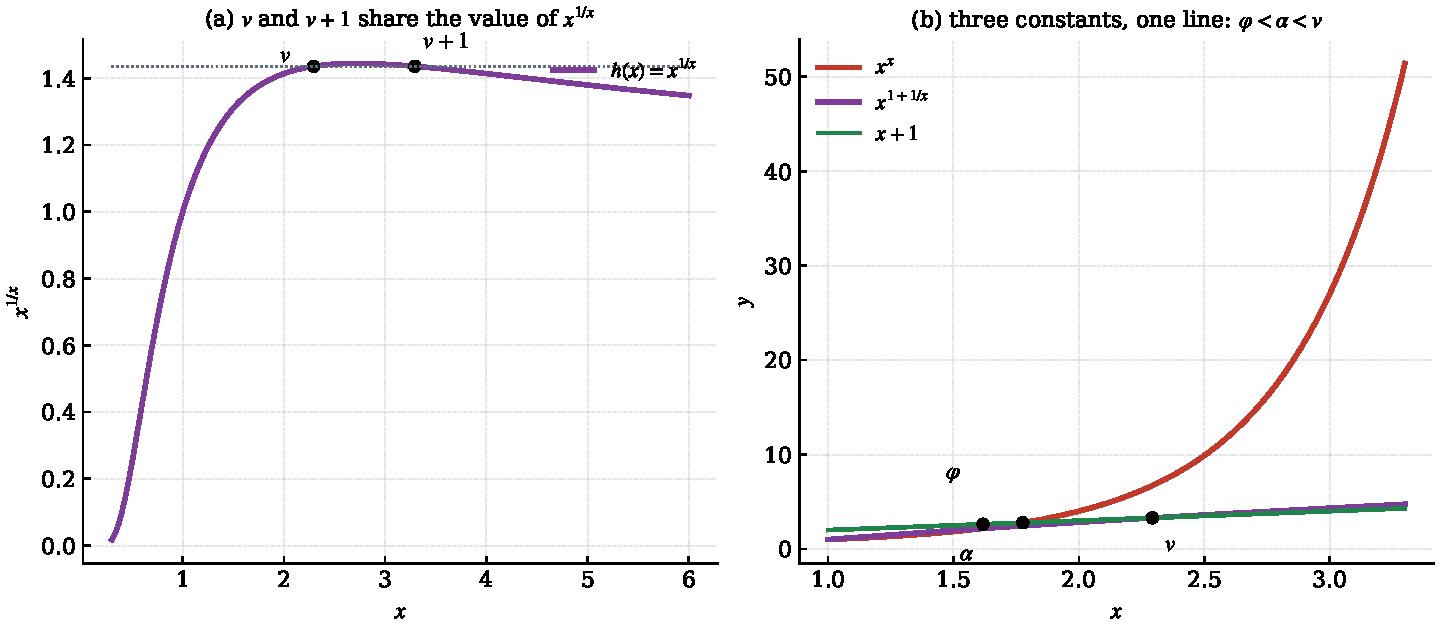
\includegraphics[width=0.98\textwidth]{figures/fig6_constants.pdf}
    \caption{(a) The map $h(x) = x^{1/x}$ is unimodal with maximum at
    $\ee$; the consecutive pair $v, v+1$ (marked, with the dotted level
    line) is the unique pair of consecutive reals on which $h$ takes
    equal values---for $h$, what the pair $(2,4)$ is classically.
    (b) The line $y = x+1$ (green), the curve $x^{x}$ (red) and the
    curve $x^{1+1/x}$ (purple): the two curves exchange order at
    $x = \varphi$ (where the exponents $x$ and $1+1/x$ coincide), the
    line is met by $x^{x}$ at $\alpha$ and by $x^{1+1/x}$ at $v$;
    consequently $\varphi < \alpha < v$, the three parameters marked
    at their heights on the line.}
    \label{fig:constants}
\end{figure}

\begin{remark}[credits and digit agreement]\label{rem:credits}
The five OEIS entries are A124930 ($\alpha$, root of $x^x = x+1$),
A226568 ($\beta$, ``the number defined by $x^x + x = 1$''), A169862
($c$, root of $x^{x-1} = (x-1)^x$), A085846 ($v$, root of
$x = (1+1/x)^x$) and A144184 ($\upsilon_2$, root of
$x^{1+1/x} = x+2$) \cite{a124930,a226568,a169862,a085846,a144184}.
Our independently computed decimal expansions of $\alpha$ and $v$ agree
digit for digit with the seventy-digit strings recorded in A124930 and
A085846, and $\beta$ agrees with the blog post's value
\cite{blog}; $c = v + 1$ and $\upsilon_2$ were verified through their
defining equations. Lord \cite{lord} proved the transcendence of $v$ by
the equivalent equation $x = (1+1/x)^{x}$; Theorem~\ref{thm:network}(v)
extends the pattern to the whole family $\upsilon_k$. The quantity
$\alpha^{\alpha-1} = 1 + 1/\alpha$ implicit in the figure, and the
identity $\beta^{\beta - 1} = (1-\beta)/\beta = v$, are the two edges
along which the constellation connects back to $\Tah$.
\end{remark}

% =====================================================================
\section{Dynamics: the attracting fixed point}\label{sec:dynamics}
% =====================================================================

Because $0 < \Tah'(y) \le 1$ everywhere with equality only at the
origin (Proposition~\ref{prop:lipschitz}), the Tahawus function is a
weak contraction of $\R$ into $(0,\infty)$, and its iteration theory
is as clean as one could hope: there is a single fixed point, it
attracts everything, and every orbit approaches it monotonically.

\begin{theorem}[fixed point]\label{thm:fixedpoint}
\begin{enumerate}[label=\textup{(\roman*)}, leftmargin=2.4em]
\item $\Tah$ has a unique fixed point
\[
    \delta \;=\; 2.2288331032781189706187615546\ldots,
    \qquad
    \delta^{\,\delta} \;=\; \delta^{2} + 1 ,
\]
which is the unique positive root of $x^{x} = x^{2}+1$ and lies in
$(2,3)$.
\item $\delta$ is transcendental.
\item Every orbit $y_{n+1} = \Tah(y_{n})$ converges to $\delta$:
strictly increasing if $y_{0} < \delta$, strictly decreasing if
$y_{0} > \delta$ (after one step from any $y_{0} \le 0$).
\item The fixed point is attracting, with
$\Tah'(\delta) = 0.2615\ldots < 1$.
\end{enumerate}
\end{theorem}

\begin{proof}
(i) For $y > 0$, $\Tah(y) = y \iff y^{y} - 1 = y^{2} \iff h(y) := y^{y}
- y^{2} - 1 = 0$; and no $y \le 0$ is fixed since $\Tah(y) > 0 \ge y$
with $\Tah(0) = 1$. Now $h < 0$ on $(0,2]$: for $0 < x < 1$,
$x^{x} < 1 < 1 + x^{2}$; for $1 \le x \le 2$, $x^{x-2} \le 1$ gives
$x^{x} \le x^{2} < x^{2}+1$. On $(2,\infty)$ write
$h(x) = x^{2}\bigl(x^{x-2} - 1 - x^{-2}\bigr)$, whose sign is the sign
of
\[
    K(x) := (x-2)\ln x - \ln\bigl(1 + x^{-2}\bigr), \qquad
    K'(x) = \ln x + \frac{x-2}{x} + \frac{2}{x(x^{2}+1)} \;>\; 0 :
\]
each term is positive for $x > 2$. Since $K(2) = -\ln\tfrac54 < 0 <
\ln 3 - \ln\tfrac{10}{9} = K(3)$, $h$ has exactly one zero
$\delta \in (2,3)$.

(iii) $\Tah(y) > y \iff h(y) < 0$ (apply the increasing $f$ to both
sides: $\Tah(y) > y \iff y = f(\Tah(y)) > f(y)$, and
$f(y) - y = h(y)/y$). So $\Tah(y) > y$ on $(0,\delta)$ and
$\Tah(y) < y$ on $(\delta,\infty)$. As $\Tah$ is increasing with
$\Tah(\delta) = \delta$, it maps $(0,\delta)$ into $(0,\delta)$ and
$(\delta,\infty)$ into $(\delta,\infty)$; monotone bounded sequences
converge, and continuity forces the limit to be a fixed point. For
$y_{0} \le 0$, $y_{1} = \Tah(y_{0}) \in (0,1] \subset (0,\delta)$.

(ii) If $\delta$ were an algebraic irrational, Gelfond--Schneider
would make $\delta^{\delta}$ transcendental, contradicting
$\delta^{\delta} = \delta^{2} + 1$ algebraic. If $\delta = p/q$ (lowest
terms, $p > q$ since $\delta > 2$), then raising
$(p/q)^{p/q} = (p^{2}+q^{2})/q^{2}$ to the $q$-th power gives
$p^{p}\, q^{\,2q-p} = (p^{2}+q^{2})^{q}$. But
$\gcd\bigl(p,\, p^{2}+q^{2}\bigr) = \gcd(p, q^{2}) = 1$, so any prime
$\ell \mid p$ has $v_\ell(\text{LHS}) = p\,v_\ell(p) > 0$ (as
$\ell \nmid q$) while $v_\ell(\text{RHS}) = 0$: impossible. Hence
$p = 1$, contradicting $p > q \ge 1$. So $\delta$ is transcendental.

(iv) $\Tah'(\delta) = \delta^{2}/f'(\delta)$ with
$f'(\delta) = \delta^{\delta-1}\bigl(\ln\delta + 1 -
\tfrac1\delta\bigr) + \delta^{-2} = 9.382\ldots$, giving
$\Tah'(\delta) = 0.2615435596\ldots$; it is $< 1$ by
Proposition~\ref{prop:lipschitz}.
\end{proof}

\begin{figure}[t]
    \centering
    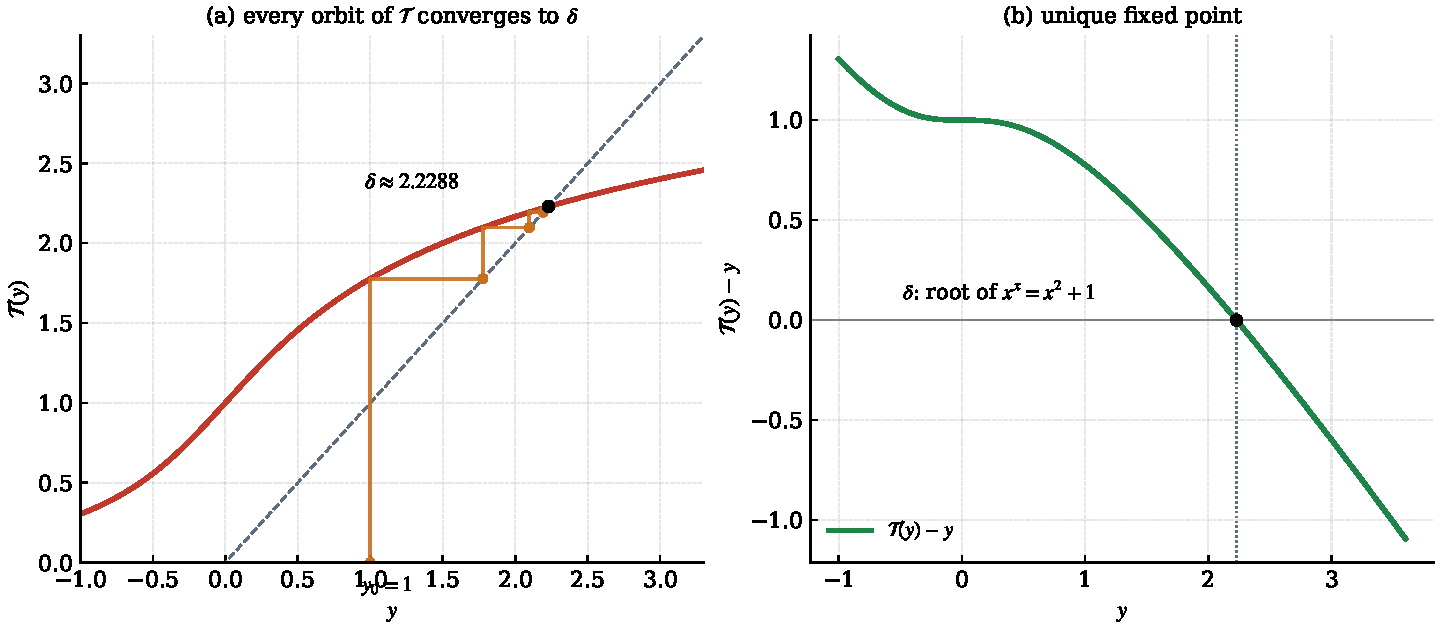
\includegraphics[width=0.98\textwidth]{figures/fig5_orbit.pdf}
    \caption{(a) Staircase diagram of the orbit of $\Tah$ started at
    $y_{0} = 1$ (orange): the orbit climbs monotonically to the
    attracting fixed point $\delta \approx 2.2288$ (black dot), where
    the graph of $\Tah$ (red) crosses the diagonal (dashed).
    (b) The displacement $\Tah(y) - y$: positive exactly on
    $(0, \delta)$, vanishing at the unique fixed point, root of
    $x^{x} = x^{2}+1$.}
    \label{fig:orbit}
\end{figure}

The orbit of $1$ is a good advertisement for the speed of the
attraction, and for how quickly the iterates forget that they started
at the Tahawus constant:
\[
\begin{aligned}
    &1,\; 1.7767750401,\; 2.0971558587,\; 2.1933551737,\;
    2.2194806484,\\
    &2.2263819619,\; 2.2281916756,\; 2.2286653182,\;
    2.2287892186,\; 2.2288216254,\;\ldots\;\to\;\delta,
\end{aligned}
\]
each step multiplying the error by roughly $\Tah'(\delta) = 0.2615$.
An orbit started at $y_{0} = -5$ reaches $0.00622$, then $1.00622$,
then follows the same staircase: one step suffices to enter
$(0,\delta)$, as promised. Newton's method on
$g(x) = x^{x} - x^{2} - 1$, started at $2$, exhibits its usual
quadratic convergence:
$2.36067$, $2.25177$, $2.22964$, $2.22883$, $2.228833103278118971$.
We remark that $\delta$ is the $n = 2$ member of the family of
\emph{super-golden} constants $\{$roots of $x^{x} = x^{n} + 1\}$,
whose first member ($n = 1$) is $\alpha$ itself; see Open
Problem~\ref{op:family}.

\subsection{The nested composition of the blog post, made convergent}
\label{subsec:W-iteration}

The infinite composition \eqref{eq:W-nest} is not a closed form, but
it \emph{is} a numerical algorithm: read from the outside in, it is
the fixed-point iteration
\begin{equation}\label{eq:W-iteration}
    x_{n+1} \;=\; \ssqrt(x_{n} + 1) \;=\; \ee^{W(\ln(x_{n}+1))},
    \qquad x_{0} \;=\; \ssqrt(2) = \ee^{W(\ln 2)},
\end{equation}
where the starting value is the first approximant obtained by ignoring
the ``$+1$'' (this is exactly the nesting displayed in the original
post). The remarkable fact is that this iteration is a
\emph{contraction with a closed-form rate}, in sharp contrast with the
power-tower iteration of the next section.

\begin{proposition}[the $W$-iteration converges geometrically]
\label{prop:W-iteration}
Let $g(x) := \ssqrt(x+1) = \ee^{W(\ln(x+1))}$ on $[0,\infty)$. Then
$g$ is increasing, $g(x) > x$ on $[0, \alpha)$, $g(x) < x$ on
$(\alpha, \infty)$, and every orbit of \eqref{eq:W-iteration}
converges monotonically to $\alpha$. Moreover $g$ is differentiable at
$\alpha$ with
\begin{equation}\label{eq:W-rate}
    g'(\alpha) \;=\; \frac{1}{(1 + \alpha)\bigl(1 + \ln \alpha\bigr)}
    \;=\; 0.2286830163\ldots \;<\; 1 ,
\end{equation}
so the convergence is geometric with ratio \eqref{eq:W-rate}.
\end{proposition}

\begin{proof}
Monotonicity of $g$ is that of $x \mapsto x + 1$, $\ln$, $W$ and
$\exp$. For $x \in [0,1)$ we have $g(x) \ge \ssqrt(1) = 1 > x$. For
$x \ge 1$ (where $t \mapsto t^{t}$ is increasing), $g(x) > x \iff
x^{x} < x + 1 \iff x < \alpha$; this uses the (known) fact that
$x^{x} - x - 1$ is strictly increasing on $[1,\infty)$, with root
$\alpha$. Hence $g$ maps $[0, \alpha]$ into $[1, \alpha]$ and
$(\alpha, \infty)$ into $(\alpha, \infty)$ with $g(x) < x$ there, and
monotone convergence proceeds exactly as in
Theorem~\ref{thm:fixedpoint}(iii), the only fixed point of $g$ in
$[0,\infty)$ being $\alpha$. For the rate:
$g'(x) = g(x)\, W'(\ln(x+1))\,/(x+1)$ with
$W'(z) = W(z)/\bigl(z(1+W(z))\bigr)$; at $x = \alpha$ we have
$g(\alpha) = \alpha$ and $W(\ln(\alpha+1)) = \ln\alpha$, because
$(\ln\alpha)\,\ee^{\ln\alpha} = \alpha\ln\alpha =
\ln(\alpha^{\alpha}) = \ln(\alpha+1)$. Substituting $z = \ln(\alpha+1)
= \alpha \ln \alpha$,
\[
    g'(\alpha)
    \;=\; \alpha \cdot \frac{\ln\alpha}{\alpha\ln\alpha\,
    (1 + \ln\alpha)} \cdot \frac{1}{\alpha + 1}
    \;=\; \frac{1}{(1+\alpha)(1+\ln\alpha)} .
    \qedhere
\]
\end{proof}

The first iterates of \eqref{eq:W-iteration} are
\[
    1.55961,\; 1.7245718243,\; 1.7646972820,\; 1.7740056666,\;
    1.7761413436,\; \ldots,\;
    1.7767750401 \;=\; \alpha ,
\]
reaching $\alpha$ to nine significant digits in eight steps; the
observed error ratios $0.23136$, $0.22930$, $0.22882$, $0.22872$,
$0.22869$, $0.228685$,~\ldots{} march to the closed form
\eqref{eq:W-rate} exactly.
This is the honest content of the blog post's nested expression: not
a closed form, but a rapidly convergent evaluation scheme. The same
scheme works verbatim for general $b$, iterating
$x \mapsto \ee^{W(\ln(bx+1))}$.

% =====================================================================
\section{The infinite power tower, corrected}\label{sec:tower}
% =====================================================================

The original post closes with a flourish: since
\begin{equation}\label{eq:blog-tower}
    \alpha^{\alpha} \;=\; \alpha + 1,
    \qquad\text{i.e.}\qquad
    \alpha^{\alpha} - 1 \;=\; \alpha ,
\end{equation}
the constant $\alpha$ can be substituted into itself forever,
\[
    \alpha \;=\; \alpha^{\alpha} - 1 \;=\;
    \alpha^{\alpha^{\alpha} - 1} - 1 \;=\;
    \alpha^{\alpha^{\alpha^{\alpha} - 1} - 1} - 1 \;=\; \cdots,
\]
an identity of infinite nested exponentials with a ``$-1$'' attached
at every level. As an \emph{algebraic} identity the chain is
unimpeachable: the sequence $x_{n+1} = \alpha^{x_{n}} - 1$ started at
$x_{0} = \alpha$ is exactly constant. As a statement about a
\emph{limit}, however---the natural reading of an infinite
expression---it is wrong, and the correction is instructive.

\begin{theorem}[the decremented tower]\label{thm:tower}
Let $1 < a < \ee$, let $g_{a}(x) := a^{x} - 1$, and let $x_{+}(a) >
0$ denote the unique positive solution of $a^{x} = x + 1$ (it exists
and is unique). Then:
\begin{enumerate}[label=\textup{(\roman*)}, leftmargin=2.4em]
\item $g_{a}$ has exactly two nonnegative fixed points, $0$ and
$x_{+}(a)$.
\item The fixed point $0$ is attracting, with multiplier
$g_{a}'(0) = \ln a < 1$; the fixed point $x_{+}(a)$ is
\emph{repelling}: its multiplier satisfies
\begin{equation}\label{eq:repelling}
    g_{a}'\bigl(x_{+}(a)\bigr) \;=\; \bigl(x_{+}(a) + 1\bigr)\ln a
    \;=\; \frac{x_{+}(a) + 1}{x_{+}(a)}\,\ln\!\bigl(x_{+}(a)+1\bigr)
    \;>\; 1 ,
\end{equation}
by the inequality $\ln(1+u) > u/(1+u)$ for $u > 0$.
\item Every orbit started in $(-1, x_{+}(a))$ converges
\emph{monotonically} to $0$; every orbit started above
$x_{+}(a)$ diverges monotonically to $+\infty$; the orbit started
exactly at $x_{+}(a)$ is stationary.
\end{enumerate}
For the Tahawus constant, $a = \alpha \in (1, \ee)$ and
$x_{+}(\alpha) = \alpha$ (this is \eqref{eq:blog-tower}), so the
decremented tower built on $\alpha$ converges to $0$ from every
starting point except $\alpha$ itself, where it is stationary, and
above which it diverges.
\end{theorem}

\begin{proof}
Put $h_{a}(x) := a^{x} - x - 1 = g_{a}(x) - x$. Then
$h_{a}(0) = 0$, $h_{a}'' = (\ln a)^{2} a^{x} > 0$, and
$h_{a}'(x) = \ln(a)\,a^{x} - 1$ is strictly increasing with
$h_{a}'(0) = \ln a - 1 < 0$ and $h_{a}' \to \infty$. So $h_a$
decreases from $h_{a}(0) = 0$ on $[0, x^{*}]$ (where $x^{*}$ is the
zero of $h_{a}'$), hence is negative on $(0, x^{*}]$, and then
increases to $+\infty$, crossing zero exactly once more at
$x_{+}(a) > x^{*}$. On $(-1, 0)$: $h_{a}$ is decreasing there (as
$(-1,0) \subset (-\infty, x^{*})$) with $h_{a}(0) = 0$, so
$h_{a} > 0$ on $(-1, 0)$: no negative fixed points; and points
$x \le -1$ are mapped into $(-1, 0)$ in one step since
$g_{a}(x) \in (-1, a^{-1} - 1] \subset (-1, 0)$. The sign of
$g_{a}(x) - x = h_{a}(x)$ is thus $+$, $-$, $+$ on the intervals
$(-1,0)$, $(0, x_{+})$, $(x_{+}, \infty)$, and $g_{a}$ maps each of
the first two intervals into itself, giving monotone convergence to
the unique fixed point of each interval, namely $0$; on the third
interval the orbit increases without fixed points above, so it
diverges. The multipliers are $g_{a}'(x) = \ln(a)\,a^{x}$: at $0$
this is $\ln a < 1$; at $x_{+}$, using $a^{x_{+}} = x_{+}+1$,
$g_{a}'(x_{+}) = (x_{+}+1)\ln a = \frac{x_{+}+1}{x_{+}}
\ln(x_{+}+1) > 1$ by $\ln(1+u) > \frac{u}{1+u}$.
\end{proof}

For $a = \alpha$ the multipliers come out as
\[
    g_{\alpha}'(0) \;=\; \ln\alpha \;=\; 0.5747999458\ldots,
    \qquad
    g_{\alpha}'(\alpha) \;=\; (1+\alpha)\ln\alpha \;=\;
    1.5960901426\ldots \;>\; 1 ,
\]
and the orbit started at $x_{0} = \tfrac12$ tells the whole story:
\[
    0.3330,\; 0.2109,\; 0.1289,\; 0.0769,\; 0.0452,\; 0.0263,\;
    0.0152,\; 0.0088,\; 0.0051,\; 0.0029,\; \ldots \;\to\; 0 ,
\]
with successive ratios $0.633, 0.611, 0.597, \ldots$ settling toward
the predicted $\ln\alpha = 0.5748$; by step $29$ the iterate is
$4.5 \times 10^{-8}$. So the corrected reading of the post's
identity is:

\begin{quote}
\emph{The decremented tower of base $\alpha$ converges---but to
$0$, not to $\alpha$. The value $\alpha$ is reachable only by the
exactly stationary (and repelling) orbit, which is an algebraic
identity, not a limit process.}
\end{quote}

Two footnotes complete the picture. First, the plain (undecremented)
tower $\alpha^{\alpha^{\alpha^{\cdots}}}$ does not converge at all:
Euler's criterion \cite{knoebel} requires the base to lie in
$[\ee^{-\ee}, \ee^{1/\ee}]$, and $\alpha = 1.7767\ldots$ exceeds
$\ee^{1/\ee} = 1.4446678\ldots$. The decrements do tame the
divergence, but the tamed limit is $0$. Second, the contrast between
Sections~\ref{subsec:W-iteration} and this one is stark and
practical: \emph{the same fixed point} $\alpha$ is repelling for the
map $x \mapsto \alpha^{x} - 1$ (multiplier $1.596$) and attracting
for the map $x \mapsto \ee^{W(\ln(x+1))}$ (multiplier $0.229$), which
are algebraically the same equation. The nest of the blog post should
always be evaluated through $W$, never through the power.

\begin{remark}[general bases]
Theorem~\ref{thm:tower} is stated for the Tahawus constant but proved
for every base $1 < a < \ee$: the pair of fixed points
$\{0, x_{+}(a)\}$ always exists, $0$ always attracts, and
$x_{+}(a)$ always repels, with \eqref{eq:repelling} holding for every
$a$. For $a \ge \ee$ even the fixed point $0$ loses stability
(multiplier $\ln a \ge 1$) and no positive fixed point exists. The
Tahawus constant is simply the special base $a$ for which the
repelling fixed point happens to \emph{coincide with the base
itself}---the self-referential charm that motivated the original
post's identity \eqref{eq:blog-tower}.
\end{remark}

% =====================================================================
\section{Asymptotics}\label{sec:asymptotics}
% =====================================================================

Both ends of the real line have clean asymptotics, and the right end
hides a surprise: at infinity the Tahawus function is a square
super-root \emph{shifted by exactly one}. Throughout, $x := \Tah(y)$,
and the starting point is an \emph{exact} identity obtained by taking
logarithms of the defining equation $x^{x} = xy + 1$ and peeling off
$\ln x$:
\begin{equation}\label{eq:master}
    x\ln x \;=\; \ln x + \ln y + \ln\Bigl(1 + \frac{1}{xy}\Bigr)
    \qquad\Longleftrightarrow\qquad
    (x - 1)\ln x \;=\; \ln y + \ln\Bigl(1 + \frac{1}{xy}\Bigr) ,
\end{equation}
the \emph{master identity on the right}. The super square root
$\ssqrt(y) = \ee^{W(\ln y)}$ of \eqref{eq:ssqrt} is the solution of
$x\ln x = \ln y$; the Tahawus function is the solution of
\eqref{eq:master}, which differs from it by the shift $x \mapsto x-1$
in the left factor and by a logarithmically tiny correction on the
right. Both differences push $x$ \emph{up} relative to $\ssqrt(y)$.

\begin{theorem}[asymptotics]\label{thm:asymptotics}
\begin{enumerate}[label=\textup{(\roman*)}, leftmargin=2.4em]
\item \emph{(far left)} As $y \to -\infty$,
\begin{equation}\label{eq:asym-left}
    \ln \Tah(y) \;=\; y - \frac{y^{2}}{2}\,\ee^{y}\bigl(1 + o(1)\bigr),
    \qquad\text{equivalently}\qquad
    \Tah(y) \;=\; \ee^{y} - \frac{y^{2}}{2}\,\ee^{2y}\bigl(1 + o(1)\bigr).
\end{equation}
\item \emph{(far right, plus-one law)} As $y \to +\infty$,
\begin{equation}\label{eq:asym-plusone}
    \Tah(y) \;-\; \ssqrt(y) \;\longrightarrow\; 1 .
\end{equation}
\item \emph{(far right, logarithmic scale)} As $y \to +\infty$,
\begin{equation}\label{eq:asym-right}
    \Tah(y) \;=\; \frac{\ln y}{\ln\ln y}
    \Bigl( 1 + \frac{\ln\ln\ln y}{\ln\ln y} +
    O\Bigl( \bigl(\tfrac{\ln\ln\ln y}{\ln\ln y}\bigr)^{2} \Bigr)
    \Bigr).
\end{equation}
\end{enumerate}
\end{theorem}

\begin{proof}
(i) Expand $f$ at $x = 0^{+}$: with $u := x \ln x \to 0$,
\[
    y \;=\; \frac{\ee^{u} - 1}{x}
    \;=\; \frac{u + \tfrac{u^{2}}{2} + O(u^{3})}{x}
    \;=\; \ln x + \frac{x\ln^{2} x}{2} + O\bigl(x^{2}\ln^{3}x\bigr) .
\]
Since $x \ln^{2} x \to 0$, we get $y - \ln x \to 0$, i.e.\
$\ln x = y + o(1)$ and $x = \ee^{y}(1 + o(1))$. Substituting back,
\[
    y - \ln x \;=\; \frac{x \ln^{2} x}{2}\bigl(1 + o(1)\bigr)
    \;=\; \frac{y^{2}}{2}\,\ee^{y}\bigl(1 + o(1)\bigr),
\]
which is \eqref{eq:asym-left}; the second form follows from
$\exp\bigl(-\tfrac{y^{2}}{2}\ee^{y}(1+o(1))\bigr) =
1 - \tfrac{y^{2}}{2}\ee^{y}(1+o(1))$, legitimate because
$\tfrac{y^{2}}{2}\ee^{y} \to 0$.

(ii) Write $L := \ln y$, let $x_{0} := \ssqrt(y) = \ee^{W(L)}$ (so
$x_{0}\ln x_{0} = L$), and let $\Phi(t) := (t-1)\ln t$, strictly
increasing on $[1, \infty)$. By \eqref{eq:master}, $x =
\Phi^{-1}(L + \varepsilon)$ with
$\varepsilon := \ln\bigl(1 + \tfrac{1}{xy}\bigr) \to 0$, while
$\Phi(x_{0} + 1) - \Phi(x_{1}) = \Phi(x_{0}+1) - L$ where $x_{1} :=
\Phi^{-1}(L)$. Now
\[
    \Phi(x_{0}+1) - L \;=\; x_{0}\ln(x_{0}+1) - x_{0}\ln x_{0}
    \;=\; x_{0}\ln\Bigl(1 + \frac{1}{x_{0}}\Bigr) \;\longrightarrow\; 1,
\]
since $x_{0} \to \infty$. By the mean value theorem there is
$\eta$ between $x_{1}$ and $x_{0}+1$ with
$(x_{0} + 1 - x_{1})\,\Phi'(\eta) = \Phi(x_{0}+1) - L \to 1$; as
$x_{0} \to \infty$ forces $\eta \to \infty$ and
$\Phi'(\eta) = \ln\eta + 1 - \tfrac1\eta \to \infty$, we conclude
$x_{1} - x_{0} \to 1$. Similarly $x - x_{1} = \Phi^{-1}(L+\varepsilon)
- \Phi^{-1}(L)$ lies between $0$ and
$\varepsilon/\Phi'(\xi) \to 0$ (mean value theorem again, with
$\xi \ge x_{1}/2 \to \infty$ for large $y$). Adding,
\[
    \Tah(y) - \ssqrt(y) \;=\; (x - x_{1}) + (x_{1} - x_{0})
    \;\longrightarrow\; 0 + 1 .
\]

(iii) From (ii) and $\ssqrt(y) = \ee^{W(L)} = L/W(L)$ it suffices to
expand $W$ at large argument: the fixed-point relation
$W = \ln L - \ln W$ iterated twice from $W_{0} = \ln L$ gives
$W(L) = \ln L - \ln\ln L + \tfrac{\ln\ln L}{\ln L}\bigl(1 +
O\bigl(\tfrac{\ln\ln L}{\ln L}\bigr)\bigr)$, whence
\[
    \frac{L}{W(L)} \;=\; \frac{L}{\ln L}\Bigl( 1 +
    \frac{\ln\ln L}{\ln L} +
    O\bigl(\bigl(\tfrac{\ln\ln L}{\ln L}\bigr)^{2}\bigr) \Bigr).
\]
Since $\Tah = \ssqrt + 1 + o(1)$ and the correction
$1 + o(1)$ is negligible against
$\tfrac{L}{\ln L} \cdot \tfrac{\ln\ln L}{\ln L} \to \infty$,
\eqref{eq:asym-right} follows with $L = \ln y$,
$\ln L = \ln\ln y$, $\ln\ln L = \ln\ln\ln y$.
\end{proof}

\begin{table}[t]
\centering
\small
\caption{Left asymptotics \eqref{eq:asym-left}: the measured
$\ln\bigl(\Tah(y)/\ee^{y}\bigr)$ against the prediction
$-\tfrac{y^{2}}{2}\ee^{y}$. By $y = -20$ the agreement is to five
significant digits.}
\label{tab:asym-left}
\begin{tabular}{rrr}
\toprule
$y$ & $\ln\bigl(\Tah(y)/\ee^{y}\bigr)$ & $-\tfrac{y^{2}}{2}\ee^{y}$ \\
\midrule
$-5$  & $-0.079444$             & $-0.084224$ \\
$-10$ & $-0.0022655$            & $-0.0022700$ \\
$-20$ & $-4.12231 \times 10^{-7}$  & $-4.12231 \times 10^{-7}$ \\
$-40$ & $-3.39868 \times 10^{-15}$ & $-3.39868 \times 10^{-15}$ \\
\bottomrule
\end{tabular}
\end{table}

\begin{table}[t]
\centering
\small
\caption{Right asymptotics: $\Tah(y)$ and the excess over the super
square root, tending to $1$ (plus-one law). The entry $T(10^{9})
\approx 10$ is explained by
$\Tah\bigl((10^{10}-1)/10\bigr) = 10$ exactly: the argument
$999{,}999{,}999.9$ is nearly $10^{9}$. The convergence in the last
column is famously slow: $\Tah - \ssqrt$ reaches only $0.74$ at
$10^{18}$, consistent with the predicted slowness of
$W(\ln y) \to \infty$.}
\label{tab:asym-right}
\begin{tabular}{rrr}
\toprule
$y$ & $\Tah(y)$ & $\Tah(y) - \ssqrt(y)$ \\
\midrule
$10^{3}$  & $5.1933138$   & $0.6377781$ \\
$10^{6}$  & $7.7478016$   & $0.6820049$ \\
$10^{9}$  & $10.0000000$  & $0.7049131$ \\
$10^{12}$ & $12.0872259$  & $0.7199081$ \\
$10^{18}$ & $15.9616322$  & $0.7393752$ \\
\bottomrule
\end{tabular}
\end{table}

Tables~\ref{tab:asym-left} and \ref{tab:asym-right} display the two
regimes; Figure~\ref{fig:growth} shows the right one on a log-log
scale, where $\Tah$ runs parallel to $\ssqrt(y) \sim \ln y/W(\ln y)$
and visibly above $\ln y$. A sharper probe of \eqref{eq:asym-plusone}:
since the shift satisfies (from the proof)
$x_{1} - x_{0} \approx W/(W+1)$ with $W = W(\ln y)$, the excess
$\Tah - \ssqrt$ should track $W(\ln y)/(W(\ln y)+1)$; at
$y = 10^{12}, 10^{24}, 10^{48}$ the pairs read
$(0.7199,\, 0.7085)$, $(0.7521,\, 0.7459)$, $(0.7792,\, 0.7759)$:
the two columns close on each other and on $1$, but only at
logarithmic speed, because $W(\ln y)$ itself grows like
$\ln\ln y$. At the googol level, $\Tah(10^{100}) = 57.7645882431$,
while the two-term formula \eqref{eq:asym-right} predicts $55.51$:
iterated logarithms converge so slowly that even a googol leaves the
third term contributing $2.3$.

\begin{figure}[t]
    \centering
    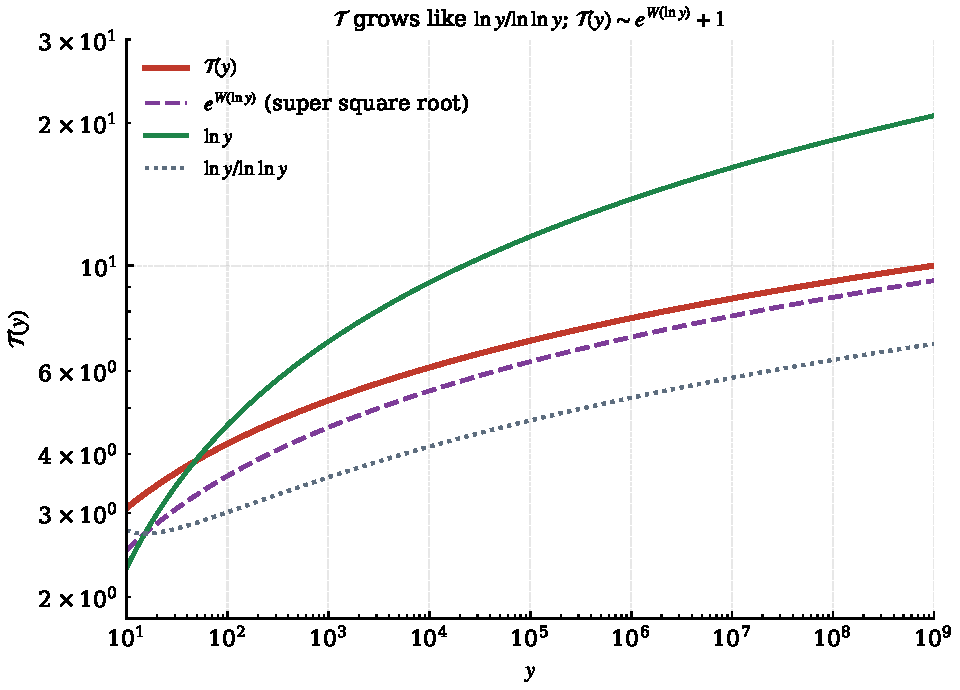
\includegraphics[width=0.78\textwidth]{figures/fig3_growth.pdf}
    \caption{Growth of $\Tah$ at large arguments (log-log scale):
    $\Tah(y)$ (solid red) runs just above the square super root
    $\ee^{W(\ln y)}$ (dashed purple), in accordance with the plus-one
    law \eqref{eq:asym-plusone}, and far below any power of $y$: its
    order is $\ln y/\ln\ln y$ (dotted curves).}
    \label{fig:growth}
\end{figure}

% =====================================================================
\section{Curiosities: integrals, a table of values, numerology, and
open problems}\label{sec:curiosities}
% =====================================================================

\subsection{Integrals}

Areas under $\Tah$ reduce, by the substitution $y = f(x)$, to areas
under $x^{x-1}$.

\begin{proposition}\label{prop:integrals}
\begin{align}
    \int_{0}^{1} \Tah(y) \dd y
    \;&=\; \alpha + \ln\alpha - \int_{1}^{\alpha} x^{x-1} \dd x
    \;=\; 1.432359924510\ldots, \label{eq:int1}\\
    \int_{-1}^{0} \bigl(1 - \Tah(y)\bigr) \dd y
    \;&=\; 1 - \beta + \ln\beta + \int_{\beta}^{1} x^{x-1} \dd x
    \;=\; 0.409721130782\ldots \label{eq:int2}
\end{align}
In \eqref{eq:int2} the integrand at the lower limit takes the value
$\beta^{\beta-1} = (1-\beta)/\beta = v$, the constant of
Theorem~\ref{thm:network}.
\end{proposition}

\begin{proof}
Substitute $y = f(x)$, $\dd y = f'(x)\dd x$. For
\eqref{eq:int1}: $\int_{0}^{1} \Tah(y) \dd y = \int_{1}^{\alpha}
x\, f'(x) \dd x = \bigl[x f(x)\bigr]_{1}^{\alpha} - \int_{1}^{\alpha}
f(x) \dd x = \alpha - \int_{1}^{\alpha}\bigl(x^{x-1} -
\tfrac1x\bigr)\dd x$. For \eqref{eq:int2}: $\int_{-1}^{0}
\bigl(1 - \Tah(y)\bigr)\dd y = \int_{\beta}^{1} (1-x) f'(x) \dd x
= \bigl[(1-x)f(x)\bigr]_{\beta}^{1} + \int_{\beta}^{1} f(x)\dd x
= (1-\beta) + \int_{\beta}^{1} x^{x-1}\dd x + \ln\beta$. The decimal
values were computed by high-precision quadrature and re-verified
through the right-hand sides.
\end{proof}

Neither $\int x^{x-1}$ nor any relative of it has a known closed
form; the classical neighbors are the two \emph{sophomore's dream}
integrals \cite{mathworld-sd},
$\int_{0}^{1} x^{-x}\dd x = \sum n^{n-1}/n!$ and
$\int_{0}^{1} x^{x} \dd x = \sum (-1)^{n+1} n^{-n}$, whose series
involve the very powers $n^{-n}$ that populate our parameters $b_n$.
Whether \eqref{eq:int1} admits an evaluation in terms of known
constants is Open Problem~\ref{op:integral}.

\subsection{A table of values}

For reference and numerical spot-checks we record
Table~\ref{tab:values}, computed to eighty significant digits and
truncated here; the exact entries are from
Proposition~\ref{prop:exactvalues} and
Theorem~\ref{thm:transcendence}, and every transcendental entry was
verified through its defining equation.

\begin{table}[t]
\centering
\small
\caption{Values of $\Tah$ at selected arguments. The entries at
$b \in \{0, \tfrac32\}$ are exact (Proposition~\ref{prop:exactvalues});
$\Tah(1) = \alpha$ and $\Tah(-1) = \beta$ are the constants of the
constellation.}
\label{tab:values}
\begin{tabular}{rll}
\toprule
$b$ & $\Tah(b)$ & remark \\
\midrule
$-10$    & $0.0000452971906610539$ & $\approx \ee^{-10}$ \\
$-5$     & $0.00622336542629749$  &  \\
$-2$     & $0.105721516538092434$ &  \\
$-3/2$   & $0.175410254005848625$ &  \\
$-1$     & $0.303659127029966051$ & $\beta$, A226568, transcendental \\
$-1/2$   & $0.556573703488657722$ &  \\
$0$      & $1$                    & exact; $=\varphi_0$ \\
$1/2$    & $1.45595925301034942$  &  \\
$1$      & $1.77677504009705470$  & $\alpha$, A124930, transcendental \\
$3/2$    & $2$                    & exact; $=\varphi_{3/2}$ \\
$2$      & $2.16575937062328429$  & partner of the root $x = -1$ \\
$\ee$     & $2.34459646238796334$ &  \\
$\pi$     & $2.42877946150189671$  &  \\
$5$      & $2.69536745976022816$  &  \\
$10$     & $3.07706224655857979$  &  \\
$100$    & $4.20694896031877337$  &  \\
$10^{6}$ & $7.74780160879762861$  &  \\
\bottomrule
\end{tabular}
\end{table}

\subsection{Numerology, debunked}

Constants as charismatic as $1.776775\ldots$ attract numerological
claims the way Tahawus attracted titanium prospectors. The
near-coincidence $\alpha \approx \sqrt{\pi}$ (they share two decimal
digits) dissolves under measurement:
\[
    \alpha - \sqrt{\pi} \;=\; 4.321189\ldots \times 10^{-3},
\]
a gap four thousand times wider than the precision to which $\alpha$
is known. A subtler trap, since it survives five digits, is
\[
    \alpha + \frac{1}{\alpha} - \bigl(\sqrt{\pi} + W(1)\bigr)
    \;=\; -4.6497 \times 10^{-6} ,
\]
and no doubt with a little effort one could manufacture coincidences
surviving eight. The theorem-level response is that
$\alpha$ is transcendental (Stanley; Corollary~\ref{cor:stanley}), so
\emph{no} identity expressing $\alpha$ through algebraic numbers can
hold exactly; identities mixing $\alpha$ with other transcendental
constants are not excluded by the theorem but are ruled out
numerically for every natural candidate we tested
($\alpha\beta = 0.5395339\ldots$, $\alpha + \beta = 2.0804341\ldots$,
$\alpha - \varphi = 0.1587410\ldots$, $1/\alpha = 0.5628174\ldots$,
none of them recognizable). The honest summary: the Tahawus constant
is a genuine constant, not a photograph of $\sqrt{\pi}$ wearing a
different hat.

\subsection{Open problems}

\begin{enumerate}[label=\textup{(\arabic*)}, leftmargin=2.2em]

\item\label{op:closedform} \textbf{No closed form.} We conjecture that
no finite expression built from the Lambert $W$ function---or from the
generalized Lambert functions of \cite{mezobaricz}---by composition,
arithmetic operations, and inversion solves the super-quadratic
$x^{x} = bx + 1$. The structural obstruction outlined in
Section~\ref{sec:background} (the unknown occurring as base, exponent,
and linearly) is not covered by any existing no-closed-form theorem
that we know of.

\item\label{op:complex-roots} \textbf{Complex roots.} How many complex
solutions does $z^{z} = z + 1$ have (per branch of the power)? By
Remark~\ref{rem:complex-roots} all of them are transcendental, but
even the count is open; nothing seems to be known about their
distribution.

\item\label{op:radius} \textbf{The radius, rigorously.} Prove that the
conjugate critical values $y_{c}, \overline{y_{c}}$ of
Subsection~\ref{subsec:radius} are the nearest singularities of the
principal branch of $\Tah$, making $R = 0.6526100\ldots$ a theorem.
The numerical evidence is strong (two independent methods, broad
critical-point sweep), but a proof requires control of all critical
values of $f$ in the disk of radius $R$.

\item\label{op:series} \textbf{The Maclaurin coefficients.} The
coefficients $d_{n}$ of \eqref{eq:maclaurin} are rational
($d_{3} = -\tfrac12$, $d_{6} = -\tfrac{49}{120},
\; d_{12} = \tfrac{62041117}{19958400}, \ldots$). Is there a closed
form, a hypergeometric-type characterization, or a generating function
for them? Is $d_{2} = 0$ the only vanishing coefficient? Do the
numerators and denominators appear in the OEIS?

\item\label{op:family} \textbf{The super-golden family.} For
$n \in \N$ let $\tau_{n}$ be the unique root of $x^{x} = x^{n} + 1$ in
$(n, n+1)$; then $\tau_{1} = \alpha$ and $\tau_{2} = \delta$, the
fixed point of Theorem~\ref{thm:fixedpoint}. The Gelfond--Schneider
step of Theorem~\ref{thm:transcendence} applies verbatim to every
$\tau_n$; what is missing is a uniform exclusion of rational roots.
Numerically $\tau_{n} = n + \bigl(n^{n}\ln n\bigr)^{-1}
\bigl(1 + o(1)\bigr)$ (already accurate to $4\%$ at $n = 3$): the
family approaches the integers super-exponentially fast. Is
$\tau_{n}$ transcendental for every $n$? We have not found
$\delta = \tau_{2}$ or any other $\tau_{n}$, $n \ge 2$, recorded in
the OEIS.

\item\label{op:tower-complex} \textbf{Complex dynamics of the
decremented tower.} Describe the Fatou/Julia dichotomy for
$z \mapsto \alpha^{z} - 1$ on the complex plane: the attracting fixed
point $0$, the repelling fixed point $\alpha$
(Theorem~\ref{thm:tower}), and the escaping set. For which bases
$a \in (1, \ee)$ does the boundary between the basin of $0$ and the
escaping set disconnect the plane?

\item\label{op:integral} \textbf{The integral.} Evaluate
$\int_{1}^{\alpha} x^{x-1}\dd x$ (equivalently
\eqref{eq:int1}) in terms of named constants or series, or prove that
no such expression exists in a reasonable class. The same question
for the moments $\int_{0}^{1} \Tah(y)^{k} \dd y$.

\end{enumerate}

The Tahawus function began life as a blog post's act of friendship
toward a beautiful unsolvable equation; we hope to have shown that it
repays systematic study. Every constant it touches---$\alpha$,
$\beta$, $v$, $\delta$---is transcendental, its graph threads between
$\ee^{y}$ and $1+y$ with third-order degeneracy at the origin, and
its inverse-functional structure ties the Lambert $W$ function, the
sophomore's dream, and the golden ratio into one small, coherent
constellation. The ghost town has a functioning mathematical namesake
at last.

% =====================================================================
\appendix
% =====================================================================

\section{Deferred elementary arguments}\label{sec:appendix}
% =====================================================================

Three small calculus facts were quoted in the body; we prove them
here. They share a theme: one-line monotonicity arguments at an
interior critical point.

\begin{lemma}\label{lem:u1}
The function $u_{1}(x) := x\bigl(1 + 2\ln x\bigr)$ satisfies
$u_{1}(x) \le 1$ on $(0, 1]$, with equality only at $x = 1$.
\end{lemma}

\begin{proof}
$u_{1}'(x) = 3 + 2\ln x$ vanishes only at $x_{0} = \ee^{-3/2}$; $u_{1}$
decreases on $(0, x_{0})$ and increases on $(x_{0}, 1]$. Hence on
$(0,1]$ its maximum is $\max\{u_{1}(x_{0}),\, u_{1}(1)\} =
\max\{-2\ee^{-3/2},\, 1\} = 1$, attained only at $x = 1$.
\end{proof}

\begin{lemma}\label{lem:q}
For $s > 0$, with $h(s) := (s-1)\ee^{-s}$:
\begin{enumerate}[label=\textup{(\roman*)}, leftmargin=2.2em]
\item $h(s) > -1$, and more precisely $h$ increases from $-1$ (at
$s \to 0^{+}$) to $h(2) = \ee^{-2}$ and then decreases back toward
$0^{+}$; in particular $h(s) \in (-1,\, \ee^{-2}]$;
\item $q(s) := (s-1)^{2}\ee^{-s} < 1$ for all $s > 0$, with
$\sup_{s>0} q(s) = \lim_{s \to 0^{+}} q(s) = 1$ not attained.
\end{enumerate}
\end{lemma}

\begin{proof}
(i) $h'(s) = (2-s)\ee^{-s}$: positive on $(0,2)$, negative on
$(2,\infty)$. So $h$ is strictly increasing from
$\lim_{s\to0^{+}} h(s) = -1$ to $h(2) = \ee^{-2}$, then strictly
decreasing with $\lim_{s\to\infty} h(s) = 0$; the range is
$(-1, \ee^{-2}]$.

(ii) $q'(s) = (s-1)(2-s)\ee^{-s}$: $q$ decreases on $(0,1)$, increases
on $(1,2)$, decreases on $(2,\infty)$, with $q(0^{+}) = 1$,
$q(1) = 0$, $q(2) = \ee^{-2} < 1$, $q(\infty) = 0$. Hence
$\sup_{s > 0} q = \max\{q(0^{+}), q(2)\} = 1$, approached only as
$s \to 0^{+}$; for every $s > 0$, $q(s) < 1$.
\end{proof}

\begin{lemma}\label{lem:logsquare}
$(\ln x)^{2} < x$ for every $x \ge 1$.
\end{lemma}

\begin{proof}
Let $k(x) := x - 2\ln x$; then $k'(x) = 1 - 2/x$ vanishes only at
$x = 2$, and $k(2) = 2 - 2\ln2 > 0$ (as $\ln 2 < 1$) with
$k \to \infty$ at both ends of $(0,\infty)$, so $k > 0$, i.e.\
$2 \ln x < x$. Now $g(x) := x - (\ln x)^{2}$ has
$g(1) = 1 > 0$ and $g'(x) = 1 - 2\ln x / x > 0$ by what was just
proved, so $g$ is increasing and positive on $[1,\infty)$.
\end{proof}

% =====================================================================
\section{Computational notes}\label{sec:computational}
% =====================================================================

All numerical statements in the paper were produced by two Python
scripts, \texttt{tahawus\_research.py} (numbers) and
\texttt{tahawus\_figures.py} (figures), delivered alongside this
article; they use \texttt{mpmath} \cite{mpmath} at $80$ significant
digits and \texttt{sympy} for the exact symbolic checks. The core
evaluator brackets the root of $x^{x} = yx + 1$ by bisection and
polishes it with Newton, robust down to the far left tail, where the
bisection is performed in $t = \ln x$:

\begin{small}
\begin{verbatim}
def f(x):  return (x**x - 1)/x

def T(y):
    y = mp.mpf(y)
    if y > 0:
        lo, hi = mp.mpf(1), mp.mpf(2)      # root in [1, inf)
        while f(hi) < y: hi *= 2
    elif y > -5:
        lo, hi = mp.mpf('1e-40'), mp.mpf(1)  # root in (0, 1]
    else:                                   # bisect in t = ln x
        tlo, thi = y - 2, mp.mpf(0)
        g = lambda t: (mp.e**(t*mp.e**t) - 1)*mp.e**(-t) - y
        for _ in range(300):
            tm = (tlo + thi)/2
            if g(tm) < 0: tlo = tm
            else:          thi = tm
        return mp.e**((tlo + thi)/2)
    for _ in range(400):                    # bisection ...
        mid = (lo + hi)/2
        if f(mid) < y: lo = mid
        else:           hi = mid
    return mp.findroot(lambda x: x**x - y*x - 1,   # ... + Newton
                       (lo, hi), tol=mp.mpf(10)**-70)
\end{verbatim}
\end{small}

The Maclaurin coefficients of Theorem~\ref{thm:maclaurin} are exact
rational numbers computed by the Lagrange--B\"urmann recurrence
\eqref{eq:lagrange} in exact arithmetic ($\mathrm{Fraction}$), with
$\varphi(u) = f(1+u)/u$ obtained by exponentiating
$E(u) = (1+u)\ln(1+u)$ by convolution, dividing by $1+u$, and
reverting:

\begin{small}
\begin{verbatim}
E = [Fr(0)]*(N+1); E[1] = Fr(1)            # (1+u)ln(1+u)
for k in range(2, N+1): E[k] = Fr((-1)**k, k*(k-1))
B = [Fr(0)]*(N+1); B[0] = Fr(1)            # exp(E), by convolutions
for k in range(1, N+1):
    B[k] = sum(i*E[i]*B[k-i] for i in range(1, k+1)) / k
phi = [F[k+1] for k in range(N)]           # phi = f(1+u)/u
inv = [Fr(1)]                              # 1/phi, by reversion
for m in range(1, N):
    inv.append(-sum(phi[i]*inv[m-i] for i in range(1, m+1)))
for n in range(1, N+1):                    # Lagrange-Buermann
    d_n = poly_pow(inv, n, trunc=n-1)[n-1] / n   # phi^{-n} at u^{n-1}
\end{verbatim}
\end{small}

\noindent The resulting $d_{1}, \ldots, d_{60}$ are those displayed in
\eqref{eq:maclaurin} (and twenty-four further exact values, used for
the radius analysis). The radius determination of
Subsection~\ref{subsec:radius} combines a least-squares fit of the
conjugate-pair recurrence $d_{n+2} = S d_{n+1} - P d_{n}$ with a direct
solve for the critical points:

\begin{small}
\begin{verbatim}
G = lambda x: x**(x+1)*(mp.log(x) + 1 - 1/x) + 1   # = x^2 f'(x)
# (1) fit (S, P) to the 60 exact d_n  ->  singularity y1 = 1/lambda
# (2) continue the inverse branch along arg(y1), then Newton on G:
xc = mp.findroot(G, (seed, seed*1.04))     # conjugate pair of roots
yc = (mp.e**(xc*mp.log(xc)) - 1)/xc        # critical value f(xc)
R  = abs(yc)                               # 0.6526100448447448
\end{verbatim}
\end{small}

\noindent The six figures are matplotlib vector PDFs (serif fonts,
identical evaluator); the scripts are reproduced in the project
directory together with the verification harness that re-checks every
numerical claim made in the text (OEIS digit strings included).
Table~\ref{tab:constants} collects the constants to sixty digits.

\begin{table}[t]
\centering
\footnotesize
\caption{Constants of the Tahawus constellation, verified to eighty
significant digits (shown truncated); see also
Table~\ref{tab:values}.}
\label{tab:constants}
\begin{tabular}{@{}ll@{}}
\toprule
constant & value \\
\midrule
$\alpha = \Tah(1)$ (A124930) & $1.776775040097054697479730744038756748637411034329296139084374\ldots$ \\
$\beta = \Tah(-1)$ (A226568) & $0.303659127029966051245018951213222659991199618761172709644170\ldots$ \\
$\delta$ (fixed point) & $2.22883310327811897061876155467799524418964882764487641840\ldots$ \\
$v = 1/\beta - 1$ (A085846) & $2.293166287411861031508028291250805864372257290327121248537710\ldots$ \\
$1/\beta$ (A169862) & $3.293166287411861031508028291250805864372257290327121248537710\ldots$ \\
$\upsilon_{2}$ (A144184) & $5.50798565277317825758902629805213873001602466330411\ldots$ \\
$\Tah(2)$ & $2.16575937062328429055689695855853100768620425410811803694712\ldots$ \\
$R$ (radius of series) & $0.652610044844744\ldots$ \\
$\Tah'(\delta)$ & $0.261543559649\ldots$ \\
$g'(\alpha) = \tfrac{1}{(1+\alpha)(1+\ln\alpha)}$ & $0.2286830163\ldots$ \\
$(1+\alpha)\ln\alpha$ (tower multiplier) & $1.5960901426\ldots$ \\
$\ln\alpha$ (multiplier at $0$) & $0.5747999458\ldots$ \\
\bottomrule
\end{tabular}
\end{table}


% =====================================================================
\begin{thebibliography}{17}\small

\bibitem{blog}
Tard\'igrados (author's pseudonym).
\emph{Hola, os presento a Tahawus: una extensi\'on de la funci\'on $W$ de
Lambert}. Blog \emph{Tard\'igrados}, 3 April 2018.
\url{https://tardigrados.wordpress.com/2018/04/03/hola-os-presento-a-tahawus-una-extension-de-la-funcion-w-de-lambert}.

\bibitem{stanley89}
R.~P. Stanley.
\emph{A transcendental number?: Quickie 88-10}.
In: Mathematical Entertainments column (S.~H. Weintraub, ed.),
\emph{The Mathematical Intelligencer} \textbf{11}, no.~1 (Winter 1989), p.~55.

\bibitem{a124930}
N.~J.~A. Sloane et al.
\emph{OEIS A124930: Decimal expansion of the unique positive real root of the
equation $x^x = x + 1$}. The On-Line Encyclopedia of Integer Sequences,
2006--2026. \url{https://oeis.org/A124930}.

\bibitem{a226568}
N.~J.~A. Sloane et al.
\emph{OEIS A226568: Decimal expansion of the number defined by $x^x + x = 1$}.
The On-Line Encyclopedia of Integer Sequences, 2013--2026.
\url{https://oeis.org/A226568}.

\bibitem{a085846}
N.~J.~A. Sloane et al.
\emph{OEIS A085846: Decimal expansion of root of $x = (1+1/x)^x$}.
The On-Line Encyclopedia of Integer Sequences, 2003--2026.
\url{https://oeis.org/A085846}.

\bibitem{a169862}
N.~J.~A. Sloane et al.
\emph{OEIS A169862: Decimal expansion of root of $x^{(x-1)} = (x-1)^x$}.
The On-Line Encyclopedia of Integer Sequences, 2010--2026.
\url{https://oeis.org/A169862}.

\bibitem{a144184}
N.~J.~A. Sloane et al.
\emph{OEIS A144184}. The On-Line Encyclopedia of Integer Sequences.
\url{https://oeis.org/A144184}.

\bibitem{corless}
R.~M. Corless, G.~H. Gonnet, D.~E.~G. Hare, D.~J. Jeffrey, D.~E. Knuth.
\emph{On the Lambert $W$ function}.
\emph{Advances in Computational Mathematics} \textbf{5} (1996), 329--359.

\bibitem{mezobaricz}
I. Mez\H{o}, \'A. Baricz.
\emph{On the generalization of the Lambert $W$ function}.
\emph{Transactions of the American Mathematical Society} \textbf{369}
(2017), 7917--7934.

\bibitem{knoebel}
R.~Arthur Knoebel.
\emph{Exponentials reiterated}.
\emph{American Mathematical Monthly} \textbf{88} (1981), 235--252.

\bibitem{gelfond}
A.~O. Gelfond.
\emph{Transcendental and Algebraic Numbers}.
Dover Publications, New York, 1960. (Gelfond--Schneider theorem, original
1934 result.)

\bibitem{lord}
Nick Lord.
\emph{Two other transcendental numbers obtained by (mis)calculating $e$}.
\emph{The Mathematical Gazette} \textbf{86}, no.~505 (2002), 103--105.

\bibitem{anghel}
Nicolae Anghel.
\emph{Foia\c{s} numbers}.
\emph{An. \c{S}tiin\c{t}. Univ.\ Ovidius Constan\c{t}a, Ser.\ Mat.}
\textbf{26}, no.~3 (2018), 21--28.

\bibitem{mactutor}
J.~J. O'Connor, E.~F. Robertson.
\emph{Richard Peter Stanley}.
MacTutor History of Mathematics archive, University of St Andrews.
\url{https://mathshistory.st-andrews.ac.uk/Biographies/Stanley/}.

\bibitem{wptahawus}
Wikipedia contributors.
\emph{Tahawus, New York}.
Wikipedia, The Free Encyclopedia.
\url{https://en.wikipedia.org/wiki/Tahawus,_New_York}.

\bibitem{mathworld-sd}
E.~W. Weisstein.
\emph{Sophomore's Dream}. From MathWorld---A Wolfram Web Resource.
\url{https://mathworld.wolfram.com/SophomoresDream.html}.

\bibitem{mpmath}
F. Johansson et al.
\emph{mpmath: a Python library for arbitrary-precision floating-point
arithmetic} (version 1.3).
\url{https://mpmath.org}.

\end{thebibliography}

\end{document}
